% ---------------------------------------------------------------------
% Real IEEE Access template (ieeeaccess.cls), sourced from the public
% erwinrmendez/ieee-access-template reference repository, which bundles
% the official class and required images (images/Logo.png,
% images/notaglineLogo.png, images/bullet.png) that this class file
% hard-codes paths to. All four files were copied to the project root.
% Front-matter macros below (\history, \doi, \address, \authorrefmark,
% \tfootnote, \markboth, \corresp, \keywords) are the class's real ones,
% not approximations.
% ---------------------------------------------------------------------
\documentclass[]{ieeeaccess}

\usepackage[T1]{fontenc}
\usepackage[utf8]{inputenc}
\usepackage{lmodern}
\usepackage{cite}
\usepackage{amsmath,amssymb,amsfonts}
\usepackage{graphicx}
\usepackage{xcolor}
\usepackage{url}
\usepackage{tabularx}
\usepackage{booktabs}
\usepackage{placeins}
\usepackage{subcaption}
\usepackage{microtype}
\usepackage[htt]{hyphenat}

\graphicspath{{figures/}{./}}
\setlength{\abovecaptionskip}{6pt plus 1pt minus 1pt}
\setlength{\belowcaptionskip}{3pt plus 1pt minus 1pt}
\setlength{\textfloatsep}{6pt plus 1pt minus 1pt}
\setlength{\floatsep}{5pt plus 1pt minus 1pt}
\setlength{\intextsep}{5pt plus 1pt minus 1pt}
\raggedbottom

\begin{document}

\vol{X}
\year{2026}
\history{Date of publication xxxx 00, 2026, date of current version xxxx 00, 2026.}
\doi{10.1109/ACCESS.2017.DOI}

\title{An AI-Ready Air-to-Ground Channel Model for HAPS--UAV Access Networks}

\author{\uppercase{Harsha Matadhikari}\authorrefmark{1}}

\address[1]{PG Diploma in Advanced Communication Engineering with Quantum AI Integration, Indian Institute of Technology Delhi, New Delhi, India (e-mail: harsha.matadhikari@gmail.com)}

\tfootnote{This work was carried out as part of the PG Diploma in Advanced Communication Engineering with Quantum AI Integration, Indian Institute of Technology Delhi.}

\markboth
{Matadhikari \headeretal: An AI-Ready Air-to-Ground Channel Model for HAPS--UAV Access Networks}
{Matadhikari \headeretal: An AI-Ready Air-to-Ground Channel Model for HAPS--UAV Access Networks}

\corresp{Corresponding author: Harsha Matadhikari (e-mail: harsha.matadhikari@gmail.com).}

\begin{abstract}
This paper develops an AI-ready air-to-ground channel model for a HAPS--UAV--Ground access network and uses it to train a learned user--platform association policy. We implement (i) a free-space and ITU-R atmospheric (rain, fog, gas, scintillation) channel model for the HAPS backhaul/feeder link (38~GHz) and the HAPS/UAV service link (2~GHz), (ii) a building-blockage line-of-sight model for the UAV access hop, and (iii) the resulting downlink SINR under a 3-HAPS equilateral-triangle constellation, including multi-HAPS co-channel interference. This channel model reveals \emph{spatial SINR heterogeneity}: at a fixed 50~km radius from the serving HAPS, SINR varies by up to 9.94~dB with receiver angle alone -- more than the 2--3~dB cost of doubling the link distance -- because of co-channel interference from the other two platforms, showing that a distance-only link budget is insufficient and motivating a learned association policy. Three rule-based policies (random, max-SINR, max-throughput) are evaluated first as baselines, confirming that association choice alone sharply affects outage and fairness. An LSTM forecasts 38~GHz feeder rain attenuation up to six hours ahead from historical weather; on held-out data it matches or beats persistence on RMSE at four-to-six-hour horizons and on MAE at five-to-six-hour horizons, and averaging the LSTM and persistence forecasts beats both alone at every horizon tested. A Deep Q-Network (DQN) agent that consumes this forecast, together with per-platform SINR, distance and battery state, learns a six-way (direct or UAV-relay, per HAPS) user--platform association policy, with the UAV relay modeled as a single static platform at a fixed position relative to the HAPS constellation rather than assumed to hover beside whichever user it serves. Across ten training experiments and 50 held-out days, the DQN is statistically indistinguishable from, and on raw reward slightly behind, the max-SINR and max-throughput rules -- a small, consistent gap traced to a higher severe-outage rate rather than to throughput, fairness or battery management, on which all three are tied. An ablation finds the LSTM forecast contributes no measurable reward benefit, and at conventional significance is slightly worse than zeroing it out. Unlike the two rule-based baselines, however, the DQN retains and uses the relay path, invoking it specifically for users already near the outage threshold (mean direct-link SINR $-1.9$\,dB when relay is chosen, against a $+2.4$\,dB population mean, consistent across all ten seeds) -- a structural capability neither baseline has, since both rest on an idealised assumption that the narrow direct-access band can serve every user at full capacity simultaneously, which does not hold at scale.
\end{abstract}

\begin{IEEEkeywords}
HAPS, UAV, non-terrestrial networks, air-to-ground channel, LoS probability, SINR, multi-node interference, UAV relay, backhaul link, rain attenuation, LSTM forecasting, deep reinforcement learning
\end{IEEEkeywords}

\titlepgskip=-15pt

\maketitle

% =====================================================================
\section{Introduction}
% =====================================================================

A High-Altitude Platform Station (HAPS) is a stratospheric, solar-powered platform at approximately 20~km altitude with a fixed service footprint of up to 100~km radius~\cite{itu_m2101,itu_m2106}. It connects to the ground over three link types:

\begin{itemize}\setlength{\itemsep}{1pt}
  \item \textbf{Service link} (HAPS to UE, 2--2.2~GHz~\cite{3gpp_ts38101_5}): direct, long-range connectivity without specialized ground hardware.
  \item \textbf{Backhaul link} (HAPS to Gateway, 38.0--39.5~GHz Ka-band, WRC-19~\cite{wrc19}): high-capacity ground-gateway connectivity.
  \item \textbf{Relay link} (HAPS to UAV to UE): a two-hop backup path for users with a poor direct link -- a 38~GHz feeder hop (HAPS--UAV, same band as the backhaul) followed by a 2~GHz access hop (UAV--UE) from a UAV hovering at lower altitude.
\end{itemize}

The 38~GHz backhaul/feeder links incur significant atmospheric loss (rain, fog, gas), while sitting in a spectral valley between the 22.235~GHz water-vapor and 60~GHz oxygen absorption resonances~\cite{itu_p676}. The 2~GHz service/relay links are resilient to atmospheric effects~\cite{itu_p618} but sensitive to building blockage. Because the 100~km service radius pushes many links to low elevation angles, slant-path lengths and the resulting atmospheric loss grow accordingly~\cite{itu_p618}.

Distance-only link budgeting, however, misses a second, larger effect: with three HAPS sharing spectrum, co-channel interference from the other two platforms makes SINR depend strongly on \emph{angular position}, not just distance. A static analysis cannot react to this, or to time-varying rain fades on the 38~GHz backhaul. This motivates an AI-ready model: a validated channel model, an LSTM rain forecaster, and a DQN agent that learns real-time user--platform association.

\textbf{Research flow.} The remainder of this paper follows three stages: (1) a \emph{channel and attenuation model} -- free-space path loss, ITU-R rain/fog/gas/scintillation, and multi-HAPS interference (\S\ref{sec:topology}--\S\ref{sec:multihaps}), characterised numerically in \S\ref{sec:results}; (2) \emph{baseline association policies} -- random, max-SINR, and max-throughput rules, evaluated on that channel model to establish how much association choice alone matters (\S\ref{sec:baseline-policies}); and (3) a \emph{learned association policy} -- an LSTM rain forecaster (\S\ref{sec:lstm}) feeding a DQN agent (\S\ref{sec:dqn}), evaluated against the stage-2 baselines (\S\ref{sec:dqn-results}).

The results follow the same three stages: (1) a reproducible ITU-R-based channel model for the HAPS, UAV and gateway links, including a quantitative characterisation of multi-HAPS interference showing where it limits the 2~GHz service link and why the 38~GHz backhaul does not, and the HAPS$\to$UAV$\to$UE relay path as an alternative to the direct service link; (2) three rule-based association baselines (random, max-SINR, max-throughput) evaluated on that model; and (3) an LSTM rain forecaster benchmarked out-of-sample against persistence, feeding a DQN association agent trained on 2024 weather and evaluated on held-out 2025 days against the stage-2 baselines.

% =====================================================================
\section{Related Work}
\label{sec:related-work}
% =====================================================================

\textbf{Building-blockage/LoS modeling (2~GHz access tier).} Holis and Pechac~\cite{holispechac2008} give the elevation-dependent building-blockage shadowing model this paper adopts for the 2~GHz HAPS/UAV access tier, originally formulated for a single serving platform with no co-channel interference term; ITU-R P.1410~\cite{itu_p1410} offers a simpler elevation-angle-only LoS baseline that the Holis--Pechac model refines with building geometry. The 38~GHz backhaul/feeder link does not need this model: the feeder hop's near-nadir geometry (the UAV sits only 0.1\,km from the serving HAPS's own nadir, \S\ref{sec:topology}) avoids building obstruction directly, while the backhaul hop (Gateway at the triangle's centroid, $\approx$27.995$^\circ$ elevation) is assumed to use a deliberately-sited, clear-sightline ground installation rather than relying on a high elevation angle for that clearance. Atmospheric loss (rain/fog/gas, \S\ref{sec:channel-models}) is the dominant impairment on both hops instead.

\textbf{Multi-HAPS co-channel interference.} Arani \emph{et al.}~\cite{arani2023} study HAPS--UAV heterogeneous networks with a DRL controller, closest in spirit to the association problem here, but evaluate a single HAPS--UAV pair with no co-channel interference term. Liu \emph{et al.}~\cite{liu2026multihaps} optimize sum-rate and worst-case SINR across multiple cooperating HAPS and ground base stations via joint user association and beamforming, but treat the channel as static and do not model time-varying rain fades or an onboard forecaster; our channel model instead quantifies the \emph{angular} SINR heterogeneity this cooperative setting would need to counteract, and complements it with the learned, weather-aware policy their static optimization does not provide.

\textbf{Contrast with Arani \emph{et al.}~\cite{arani2023}.} Because this is the closest prior work, we make the delta explicit. (i) \emph{Interference:} their DRL controller is evaluated on a single HAPS--UAV pair, so it has no co-channel term to learn around; our 3-HAPS geometry shows angular position alone swings SINR by 9.94\,dB at fixed range (\S\ref{sec:multihaps}), a degree of freedom their setting cannot expose. (ii) \emph{Weather coupling:} their feeder/access channel is time-invariant, so the controller cannot anticipate fades; our DQN consumes a six-horizon LSTM rain forecast (\S\ref{sec:lstm}) specifically because the feeder link is not static. (iii) \emph{Reward structure:} we jointly penalize outage, fairness, and per-platform battery depletion (\S\ref{sec:dqn}, Eq.~\eqref{eq:reward}) in a single reward, rather than optimizing throughput alone, so the comparison against rule-based max-throughput/max-SINR baselines (\S\ref{sec:dqn-results}) isolates what the extra state (forecast, battery, fairness) buys over a narrower throughput-only objective.

\textbf{Learned resource allocation and association in NTN.} Naous \emph{et al.}~\cite{naous2023rlsky} survey reinforcement learning across non-terrestrial platforms (satellites, HAPS, UAVs) and note that most RL-based association work either assumes a static channel or omits weather-driven feeder-link variability -- the gap this paper's LSTM-fed DQN targets. Foundational DQN~\cite{mnih2015dqn} and RL theory~\cite{sutton2018rl} underpin the agent design of \S\ref{sec:dqn}; PPO~\cite{schulman2017ppo} was considered but DQN suits this paper's small discrete (six-action) space better, at lower sample complexity. Fairness is quantified with the Jain index~\cite{jain1984quantitative}, and per-link SINR is combined in the linear domain following standard practice~\cite{goldsmith2005} rather than by averaging in dB.

\textbf{Rain attenuation forecasting.} Cornejo \emph{et al.}~\cite{cornejo2022lstmrain} train an LSTM on synthetic, ITU-R-derived rain-attenuation traces for satellite links, reporting improved short-term prediction accuracy over classical models; this paper instead trains on several years of real, multi-source weather data (NASA POWER, METAR, ERA5, 2023--2026) for a specific HAPS feeder-link geometry and benchmarks against a persistence baseline, which (\S\ref{sec:lstm}) proves non-trivial to beat at short horizons. The resulting rain margins are consistent with the Ka-band FSS rain-margin guidance in ECC Report 156~\cite{ecc_report_156} (\S\ref{subsec:backhaul-model}).

\textbf{Survey context.} The recent survey by Svistunov \emph{et al.}~\cite{svistunov2025haps} catalogs HAPS channel modeling, interference control, and AI-driven resource allocation at a high level, and the broader survey by Bakambekova \emph{et al.}~\cite{bakambekova2024} on AI for space-air-ground integrated networks identifies weather-aware, cross-layer learning as an open direction at the SAGIN level; this paper provides one of the quantitative instances -- a validated channel model and a trained, evaluated association policy -- that both surveys point to as needed.

\textbf{Positioning.} None of the above combines all three elements this paper does: (i) an ITU-R-validated, multi-HAPS interference-aware channel model showing that angular position can dominate distance in SINR, (ii) an out-of-sample rain forecaster feeding (iii) a DQN association policy evaluated against rule-based baselines on real held-out weather. This combination, rather than any single component in isolation, is the contribution.

% =====================================================================
\section{System Topology and Channel Model}
\label{sec:topology}
% =====================================================================

\begin{table}[t]
\centering
\caption{Simulated network configuration (AGL = above ground level)}
\label{tab:config}
{\scriptsize\setlength{\tabcolsep}{3pt}
\begin{tabularx}{\columnwidth}{|>{\raggedright\arraybackslash}X|>{\raggedright\arraybackslash}X|>{\centering\arraybackslash}X|>{\raggedright\arraybackslash}X|}
\hline
\textbf{Node} & \textbf{Altitude} & \textbf{Count} & \textbf{Spacing} \\
\hline
HAPS & 20\,km & 3 & Equilateral 65\,km, 1 server, 2 interferers \\
\hline
UAV relay & 500\,m AGL & 1 & Static, fixed 0.1\,km from serving HAPS nadir, good-sector azimuth (no mobility) \\
\hline
Gateway & 50\,m AGL & 1 & Centroid of HAPS triangle \\
\hline
Users & 1.5\,m (hand-held) & $N$ (configurable) & Uniform random in coverage \\
\hline
\end{tabularx}}
\end{table}

\begin{figure}[t]
\centering
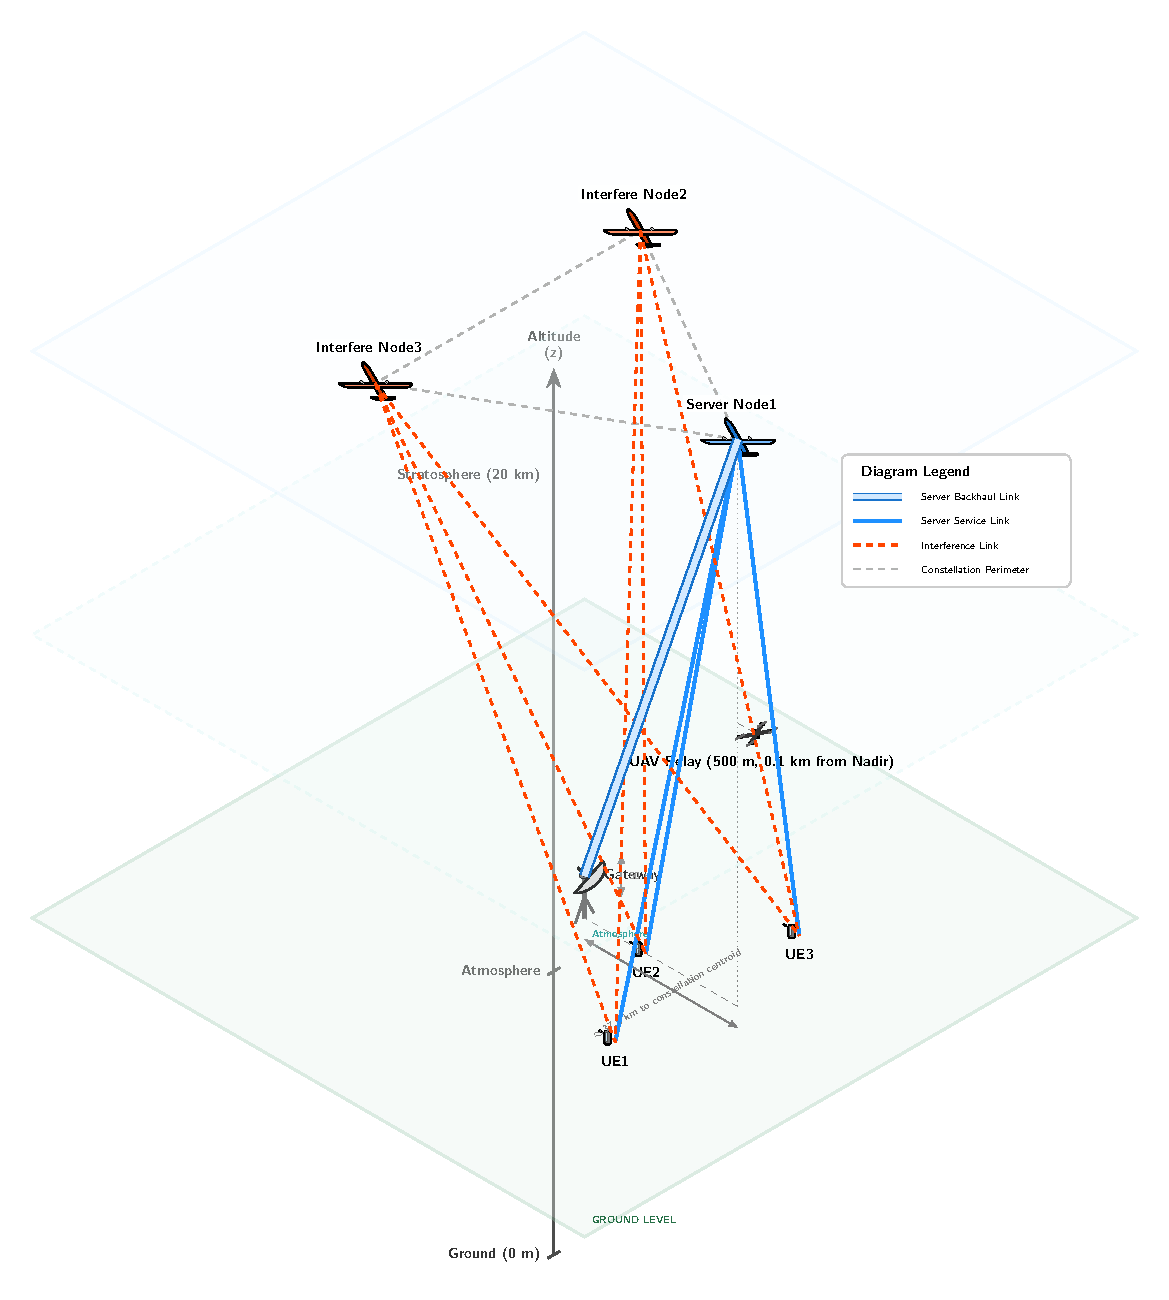
\includegraphics[width=0.9\linewidth]{./figures/network_diagram_gw.pdf}
\caption{Network topology: three HAPS nodes and one UAV relay serve ground users over an access layer; a single ground gateway aggregates the backhaul links into the core network.}
\label{fig:simulation-topology}
\end{figure}

Three HAPS nodes and one UAV relay serve ground users (access layer); a single ground gateway aggregates all three backhaul links (backhaul layer) into the core network (Table~\ref{tab:config}, Fig.~\ref{fig:simulation-topology}). Elevation angle and slant-path length follow directly from each link's altitude pair and horizontal offset: the backhaul link (HAPS to a Gateway fixed at the triangle's centroid) is at a much shallower $\approx$27.995$^\circ$, while the HAPS--UAV feeder hop (UAV fixed 0.1\,km from the serving HAPS's own nadir) is near-zenith ($\approx$89.71$^\circ$); the UAV--UE access hop is dominated by horizontal offset and building blockage rather than altitude; and the direct HAPS--UE service link spans the full service radius, from near-zenith at nadir to low elevation at the 100~km edge.

\textbf{Channel model.} Three propagation models apply to this topology: (i) free-space path loss (FSPL), common to all links; (ii) ITU-R rain, fog, gas and scintillation losses, applicable to the 38~GHz backhaul and feeder links; and (iii) a building-blockage LoS/NLoS probability model (Holis \& Pechac~\cite{holispechac2008}), applicable to the 2~GHz UAV/HAPS access-tier links.

The ITU-R P.530 free-space path loss~\cite{itu_p530} is
\begin{equation}
L_\mathrm{FSPL} = 32.44 + 20\log_{10} f_\mathrm{MHz} + 20\log_{10} d_\mathrm{km} \;[\mathrm{dB}],
\label{eq:fspl}
\end{equation}
where $f_\mathrm{MHz}$ is the carrier frequency and $d_\mathrm{km}$ the link distance. This is algebraically the wavelength form $L_\mathrm{FSPL}(h,r)=20\log_{10}(4\pi d_{h,r}/\lambda)$ used later in the multi-HAPS SINR formulation (\S\ref{sec:multihaps}): substituting $\lambda=c/f$ and converting units folds the resulting constant into the $32.44$\,dB term above.

% =====================================================================
\section{Atmospheric and Propagation Models}
\label{sec:channel-models}
% =====================================================================

\subsection{38~GHz Backhaul/Feeder Link}
\label{subsec:backhaul-model}

Rain attenuation $\gamma_R$ (dB/km) follows the ITU-R P.838 power law~\cite{itu_p838}
\begin{equation}
\gamma_R = k(f,\theta)\,R^{\alpha(f,\theta)} \quad [\mathrm{dB/km}],
\label{eq:rain_spec_atten}
\end{equation}
with $k\approx0.398$, $\alpha\approx0.879$ at 38~GHz for the Gateway's centroid ($\approx27.995^\circ$) geometry (horizontal polarisation), giving $\gamma_R\approx3.0$\,dB/km at 10\,mm/h and $\approx6.7$\,dB/km at 25\,mm/h. Multiplying by the ITU-R P.618 effective slant length $L_\mathrm{eff}$~\cite{itu_p618} gives $A_\mathrm{rain}=\gamma_R L_\mathrm{eff}$. For Delhi's $R_{0.1}=15.7$\,mm/h rain rate (ITU-R P.837~\cite{itu_p837}), this gives $\approx8.6$\,dB of rain loss on the Gateway's centroid path. Against the clear-sky backhaul SINR of $\approx+39.9$\,dB (\S\ref{sec:multihaps}) and $\approx0.4$\,dB of additional gas loss, the resulting link margin is $39.9-8.6-0.4\approx30.9$\,dB at 99.9\,\% availability -- well above the 15--25\,dB Ka-band rain margins reported for FSS links by ECC Report 156~\cite{ecc_report_156}, and a much larger margin than the previous near-nadir Gateway geometry's $\approx18.6$\,dB, because the longer, shallower slant path through the rain layer is de-rated more strongly by the P.618 reduction factor -- so the 38~GHz backhaul therefore closes comfortably at the design availability target.

Fog/cloud loss (ITU-R P.840~\cite{itu_p840}) and gas absorption (ITU-R P.676~\cite{itu_p676}) are modeled as specific attenuations times slant length, $A_\mathrm{cloud}=\gamma_c(f,M,T)L_\mathrm{slant}$ and $A_\mathrm{gas}=(\gamma_o+\gamma_w)L_\mathrm{slant}$; both are small at 38~GHz (fog typically $<0.2$\,dB; clear-sky gas $\approx0.2$--$0.3$\,dB/km, versus $\sim$15--20\,dB/km at the 60~GHz oxygen resonance). Tropospheric scintillation (ITU-R P.618 Annex~1~\cite{itu_p618}) is
\begin{equation}
A_\mathrm{scint}(p) = a(p)\cdot\sigma_\mathrm{pre}(f,\theta,\mathrm{climate}) \quad [\mathrm{dB}],
\label{eq:scint_loss}
\end{equation}
growing with frequency and shrinking with elevation. Total backhaul/feeder slant-path attenuation sums all terms:
\begin{equation}
L_\mathrm{total} = L_\mathrm{FSPL} + A_\mathrm{rain} + A_\mathrm{cloud/fog} + A_\mathrm{gas} + A_\mathrm{scint}.
\label{eq:feeder_loss}
\end{equation}

\subsection{2~GHz Service/Relay Link}
\label{subsec:service-model}

Unlike the 38~GHz links, the 2~GHz band is resilient to atmospheric effects but sensitive to building blockage. For a UAV or HAPS node $u$ at horizontal distance $r_{u,k}$ from user $k$, the LoS probability follows the building-blockage product series of Arani et al.~\cite{arani2023}, parameterised by Holis \& Pechac~\cite{holispechac2008}:
\begin{equation}
P^\mathrm{LoS}_{u,k} = \prod_{n=0}^{J}\left[1-\exp\!\left(-\frac{1}{2\xi^2}\Big(h_u-\tfrac{n+\frac12}{J+1}(h_u-h_k)\Big)^{2}\right)\right],
\label{eq:los}
\end{equation}
with $J=\lfloor \tfrac{r_{u,k}}{1000}\sqrt{\alpha\beta}-1\rfloor$ building layers, and environment-dependent parameters $(\alpha,\beta,\xi)$ (e.g.\ suburban $0.1,750,8$\,m; urban $0.3,500,15$\,m; dense urban $0.5,300,20$\,m; high-rise $0.5,300,50$\,m)~\cite{holispechac2008}. This single-relay topology (Table~\ref{tab:config}) needs only a 3-HAPS interference sum; no UAV-to-UAV term is required.

Each propagation state $z\in\{\mathrm{LoS,NLoS}\}$ adds a log-normal shadowing term, averaged in linear gain (not dB, since the two states can differ by up to $\sim$17\,dB in dB-domain averaging):
\begin{align}
\overline{g} &= 10^{-\mathrm{FSPL}/10}\Big[P_\mathrm{LoS}\,e^{\tfrac{(a\sigma_\mathrm{LoS})^2}{2}} + P_\mathrm{NLoS}\,e^{-a\mu(\theta)+\tfrac{(a\sigma(\theta))^2}{2}}\Big],\nonumber\\
\overline{\mathrm{PL}} &= -10\log_{10}\overline{g}, \qquad a=\tfrac{\ln 10}{10}.
\label{eq:pl}
\end{align}
The downlink SINR at user $k$ from node $u$ is then
\begin{equation}
\gamma_{u,k} = \frac{p_u\,g_{u,k}}{\sum_{u'\neq u} p_{u'} g_{u',k} + \sigma_0^2}, \qquad g_{u,k}=10^{-\overline{\mathrm{PL}}/10}.
\label{eq:sinr}
\end{equation}

% =====================================================================
\section{Multi-HAPS Interference, SINR, and the Relay Path}
\label{sec:multihaps}
% =====================================================================

With three HAPS sharing spectrum, a serving HAPS $h$ provides the desired signal while the other two contribute co-channel interference at the same receiver $r$ (gateway, UAV, or UE):
\begin{equation}
\gamma_{h,r}=\frac{P_hG_hG_r g_{h,r}}{N_r + \displaystyle\sum_{h'\neq h}P_{h'}G_{h'}G_r g_{h',r}},
\label{eq:general-haps-sinr}
\end{equation}
with channel gain $g_{h,r}=10^{-L_{h,r}^\mathrm{tot}/10}$ from the total propagation loss of \S\ref{sec:channel-models}. This same formulation instantiates the backhaul link ($r=$ gateway), the feeder hop ($r=$ UAV), and the direct service link ($r=$ UE); the UAV--UE access hop uses UAV transmitters/receivers in place of HAPS and is interference-free with a single relay.

\textbf{Backhaul link.} The gateway is fixed at the HAPS triangle's centroid, so it is equidistant ($\approx$42.50\,km slant) from the serving HAPS \emph{and} both interfering HAPS. Despite the equal distance, each interferer's main beam points at its own service area rather than at the centroid ($\approx62^\circ$ off its own nadir), and the gateway's own dish points at the serving HAPS, so each interferer is seen $\approx100^\circ$ off the gateway's boresight -- both fall on the ITU-R F.699 sidelobe floor ($-10$\,dBi). With directional antenna gains included ($G_h=13.8$\,dBi, $G_g=39.7$\,dBi~\cite{karaman2025haps}), the interference term is $\approx-31$\,dB below the noise floor, so the backhaul SINR is $\approx+39.9$\,dB and \textbf{noise-limited}.

\textbf{Feeder hop (HAPS$\to$UAV).} With the single relay UAV fixed 0.1\,km from the serving HAPS's own nadir (\S\ref{sec:relay-path-analysis}) rather than tracking the user, this hop has one \textbf{constant} geometry regardless of distance or which HAPS relays: $\approx$89.71$^\circ$ elevation, noise-limited at $+37.6$\,dB, using $G_h=13.8$\,dBi and a UAV-mountable mmWave patch array $G_u=30.7$\,dBi~\cite{anim2021uav}.

\textbf{Service link (HAPS$\to$UE).} Here the picture is different. A receiver at horizontal distance $r$ from the serving HAPS's nadir and the two interferers at $\approx$65~km produces an \textbf{angularly-dependent} SINR: at a fixed $r=50$\,km, SINR ranges from $-7.40$\,dB toward an interferer ($\theta=0^\circ$) to $+2.54$\,dB away from the constellation ($\theta=210^\circ$) -- a $9.94$\,dB spread -- mapping to a good sector ($\approx$120$^\circ$--290$^\circ$) and a bad sector ($\approx$330$^\circ$--75$^\circ$) (Fig.~\ref{fig:app-constellation-sectors}, \S\ref{sec:results}). Averaged over all azimuths, mean service-link SINR falls from $+6.3$\,dB at 10\,km to $-4.3$\,dB at 100\,km, while the angular min--max band widens from 1.95\,dB to a peak of 11.94\,dB at 75\,km (Fig.~\ref{fig:multinode-interference}, \S\ref{sec:results}) -- beyond $\sim$30\,km, angular position dominates over distance decay. This spread (9.94\,dB at fixed distance) exceeds the $\sim$2--3\,dB cost of simply doubling the link distance, so a distance-only link budget cannot characterise the interference environment, and the network needs TDMA/FDMA/beamforming/power control, or a learned association policy, to manage it.

\subsection{Relay Path Analysis (HAPS$\to$UAV$\to$UE)}
\label{sec:relay-path-analysis}

The relay path's end-to-end capacity is the decode-and-forward bottleneck of its two hops, $C_\mathrm{relay}=\min(C_\mathrm{haps-uav},C_\mathrm{uav-ue})$. The single relay UAV (Table~\ref{tab:config}) is static, fixed 0.1\,km from the serving HAPS's own nadir rather than hovering beside whichever user it serves -- the only placement consistent with "static" and with there being one UAV to assign (\S\ref{sec:dqn}); the Gateway now occupies the centroid instead (circumradius $65/\sqrt{3}\approx37.5$\,km from each HAPS). So the feeder hop (HAPS$\to$UAV) has one \textbf{constant} elevation ($\approx$89.71$^\circ$) and capacity ($12.48$\,bits/s/Hz) regardless of which HAPS relays or which user is served. The access hop (UAV$\to$UE, 2\,GHz) instead depends on each user's real horizontal distance from this one fixed point: capacity falls from $11.1$\,bits/s/Hz at the UAV's own location to $0.96$\,bits/s/Hz at 5\,km and $0.17$\,bits/s/Hz at 10\,km (urban terrain -- unchanged from the previous centroid-UAV geometry, since the access-hop model depends only on the UAV's altitude and sweep distance, not on where the UAV sits relative to the HAPS triangle), collapsing far faster than the direct HAPS$\to$UE link does over the same distances because the UAV's 500\,m altitude loses elevation -- and so LoS probability -- much sooner than a 20\,km-altitude HAPS does. The usable-relay radius, where access-hop capacity crosses a $0.5$\,bits/s/Hz floor, is $\approx6.5$\,km, also essentially unchanged. However, because the feeder hop's capacity ($12.48$) now exceeds the access hop's own peak ($11.1$ at the UAV), the access hop is the bottleneck even at the UAV itself, unlike before; and because the UAV's disk now sits right next to the serving HAPS's own nadir rather than 37.5\,km away, averaged over azimuth around the serving HAPS, relay capacity now \emph{exceeds} the direct link's within about 1--2\,km of the serving HAPS's nadir (urban terrain), rather than never, as under the previous centroid-UAV geometry -- but it still falls back below the direct link for the rest of the $6.5$\,km disk, so averaged over the \emph{whole} disk the relay now delivers less area-averaged capacity than the direct link does over that same disk ($\approx0.79\times$, urban), not more. The relay therefore helps only the small fraction of users within this radius of the one fixed UAV, not every user -- a single static platform cannot be close to everyone across a 100\,km-radius footprint; \S\ref{sec:conclusion} quantifies how many additional, well-placed UAVs this implies. This motivates including the UAV relay as an association option for the learned policy of \S\ref{sec:dqn}, which (\S\ref{sec:dqn-results}) learns to invoke it only for users it actually helps.

% =====================================================================
\section{Simulation Results}
\label{sec:results}
% =====================================================================

All results use a Python simulation stack (\texttt{NumPy}/\texttt{pandas}/\texttt{Matplotlib}); atmospheric and scintillation losses use the ITU-Rpy (\texttt{itur})~\cite{itur_package} library's implementation of the relevant ITU-R recommendations.

\subsection{Why 38~GHz: Frequency Selection}

This subsection validates the 38~GHz backhaul/feeder choice already fixed in \S\ref{sec:topology} (WRC-19 allocation). It is included to address a natural reader question: why not simply pick a lower-loss frequency instead of designing around rain, fog, and gas attenuation at 38~GHz?

\begin{figure}[!t]\centering
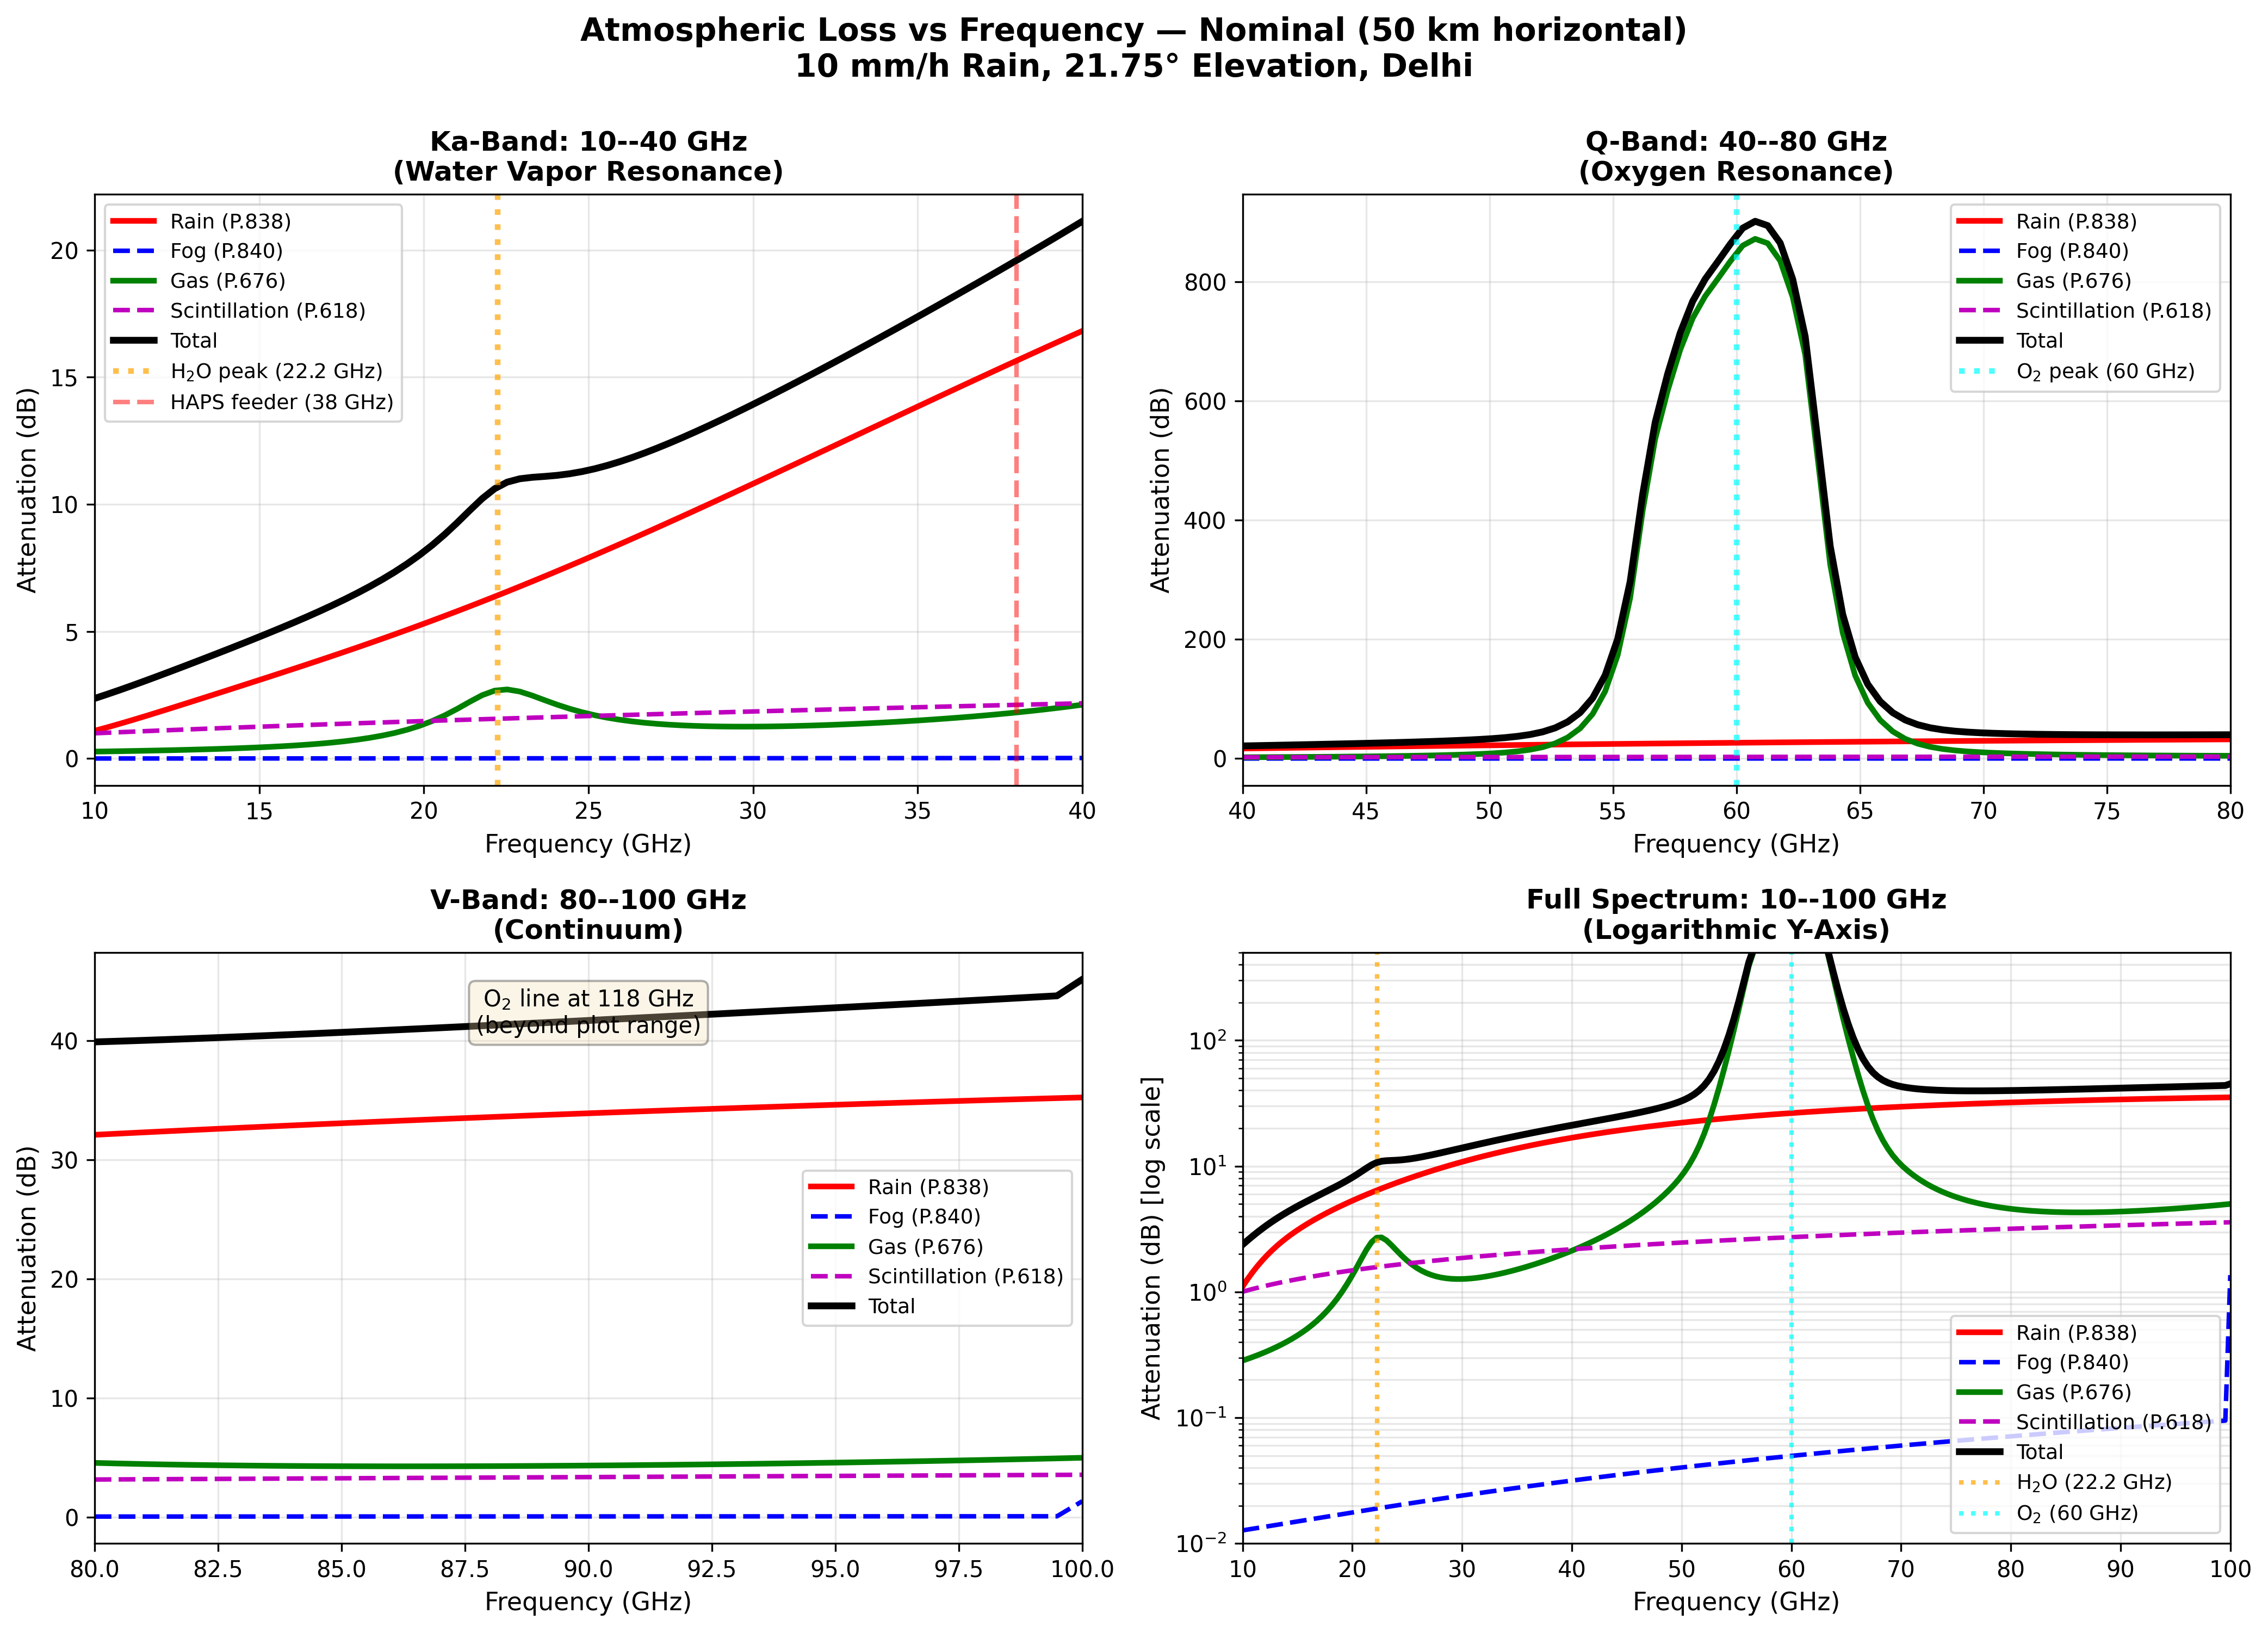
\includegraphics[width=0.95\columnwidth]{./figures/fig_atm_loss_nominal_frequency.png}
\caption{Atmospheric loss (rain, fog, gas) vs.\ frequency across the Ka/Q/V bands for the Delhi gateway path at 10\,mm/h rain.}
\label{fig:atm_frequency_nominal}
\end{figure}

Rain loss (ITU-R P.838/P.618~\cite{itu_p838,itu_p618}) is the dominant term and grows roughly linearly with frequency, up to $\approx$19\,dB at 99.9\,\% availability. Fog/cloud (ITU-R P.840~\cite{itu_p840}) is negligible below 10~GHz. Gas absorption (ITU-R P.676~\cite{itu_p676}) has two resonance peaks to avoid: water vapor at 22.2~GHz and oxygen at 60~GHz, where total loss exceeds 800\,dB over 50\,km and the band is unusable. \textbf{38~GHz sits in the valley between these peaks} ($\approx$0.2--0.3\,dB/km clear-sky gas loss) -- this, not just available bandwidth, is why it was chosen over a frequency closer to either resonance.

\subsection{Path Loss and SINR vs.\ Distance}

\begin{figure}[!t]\centering
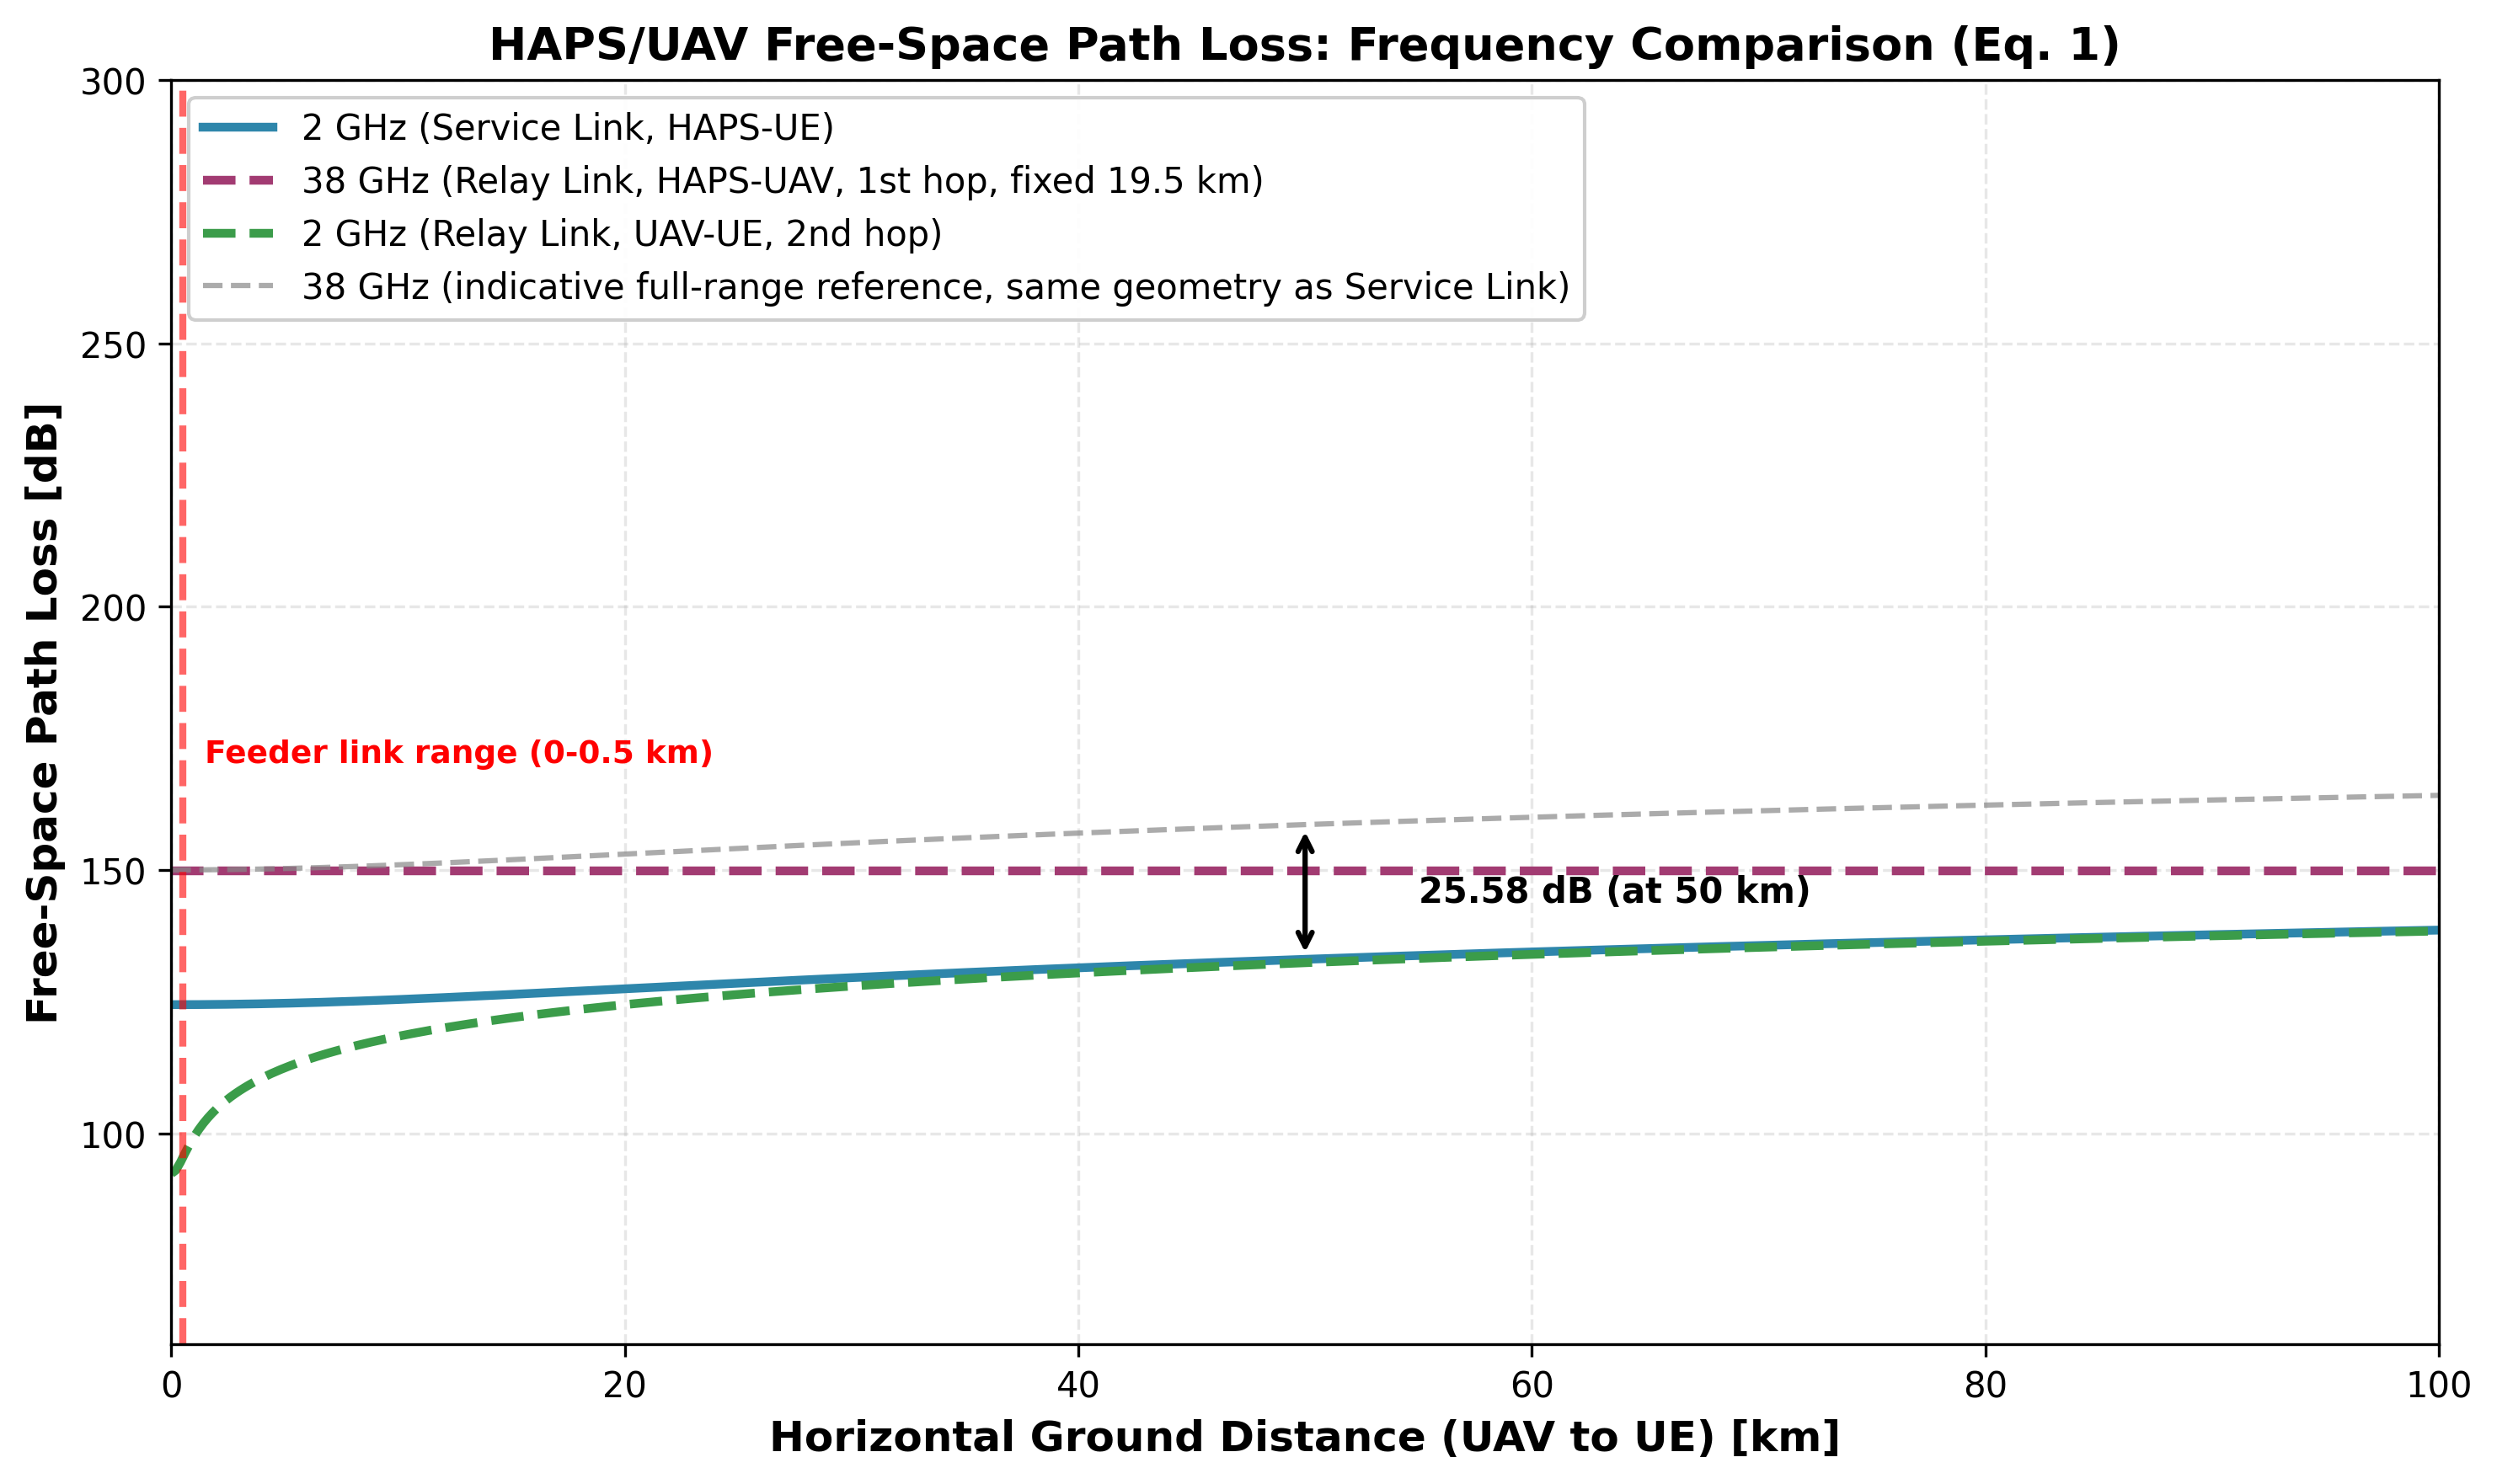
\includegraphics[width=0.95\columnwidth]{./figures/1b_haps_fspl_2ghz_vs_38ghz.png}
\caption{FSPL vs.\ distance (Eq.~\eqref{eq:fspl}) -- same functional form for 2 and 38~GHz; the 38~GHz feeder sits $\approx$25.6\,dB higher, purely from the $20\log_{10}(38/2)$ frequency term.}
\label{fig:fspl_comparison}
\end{figure}

\begin{figure}[!t]\centering
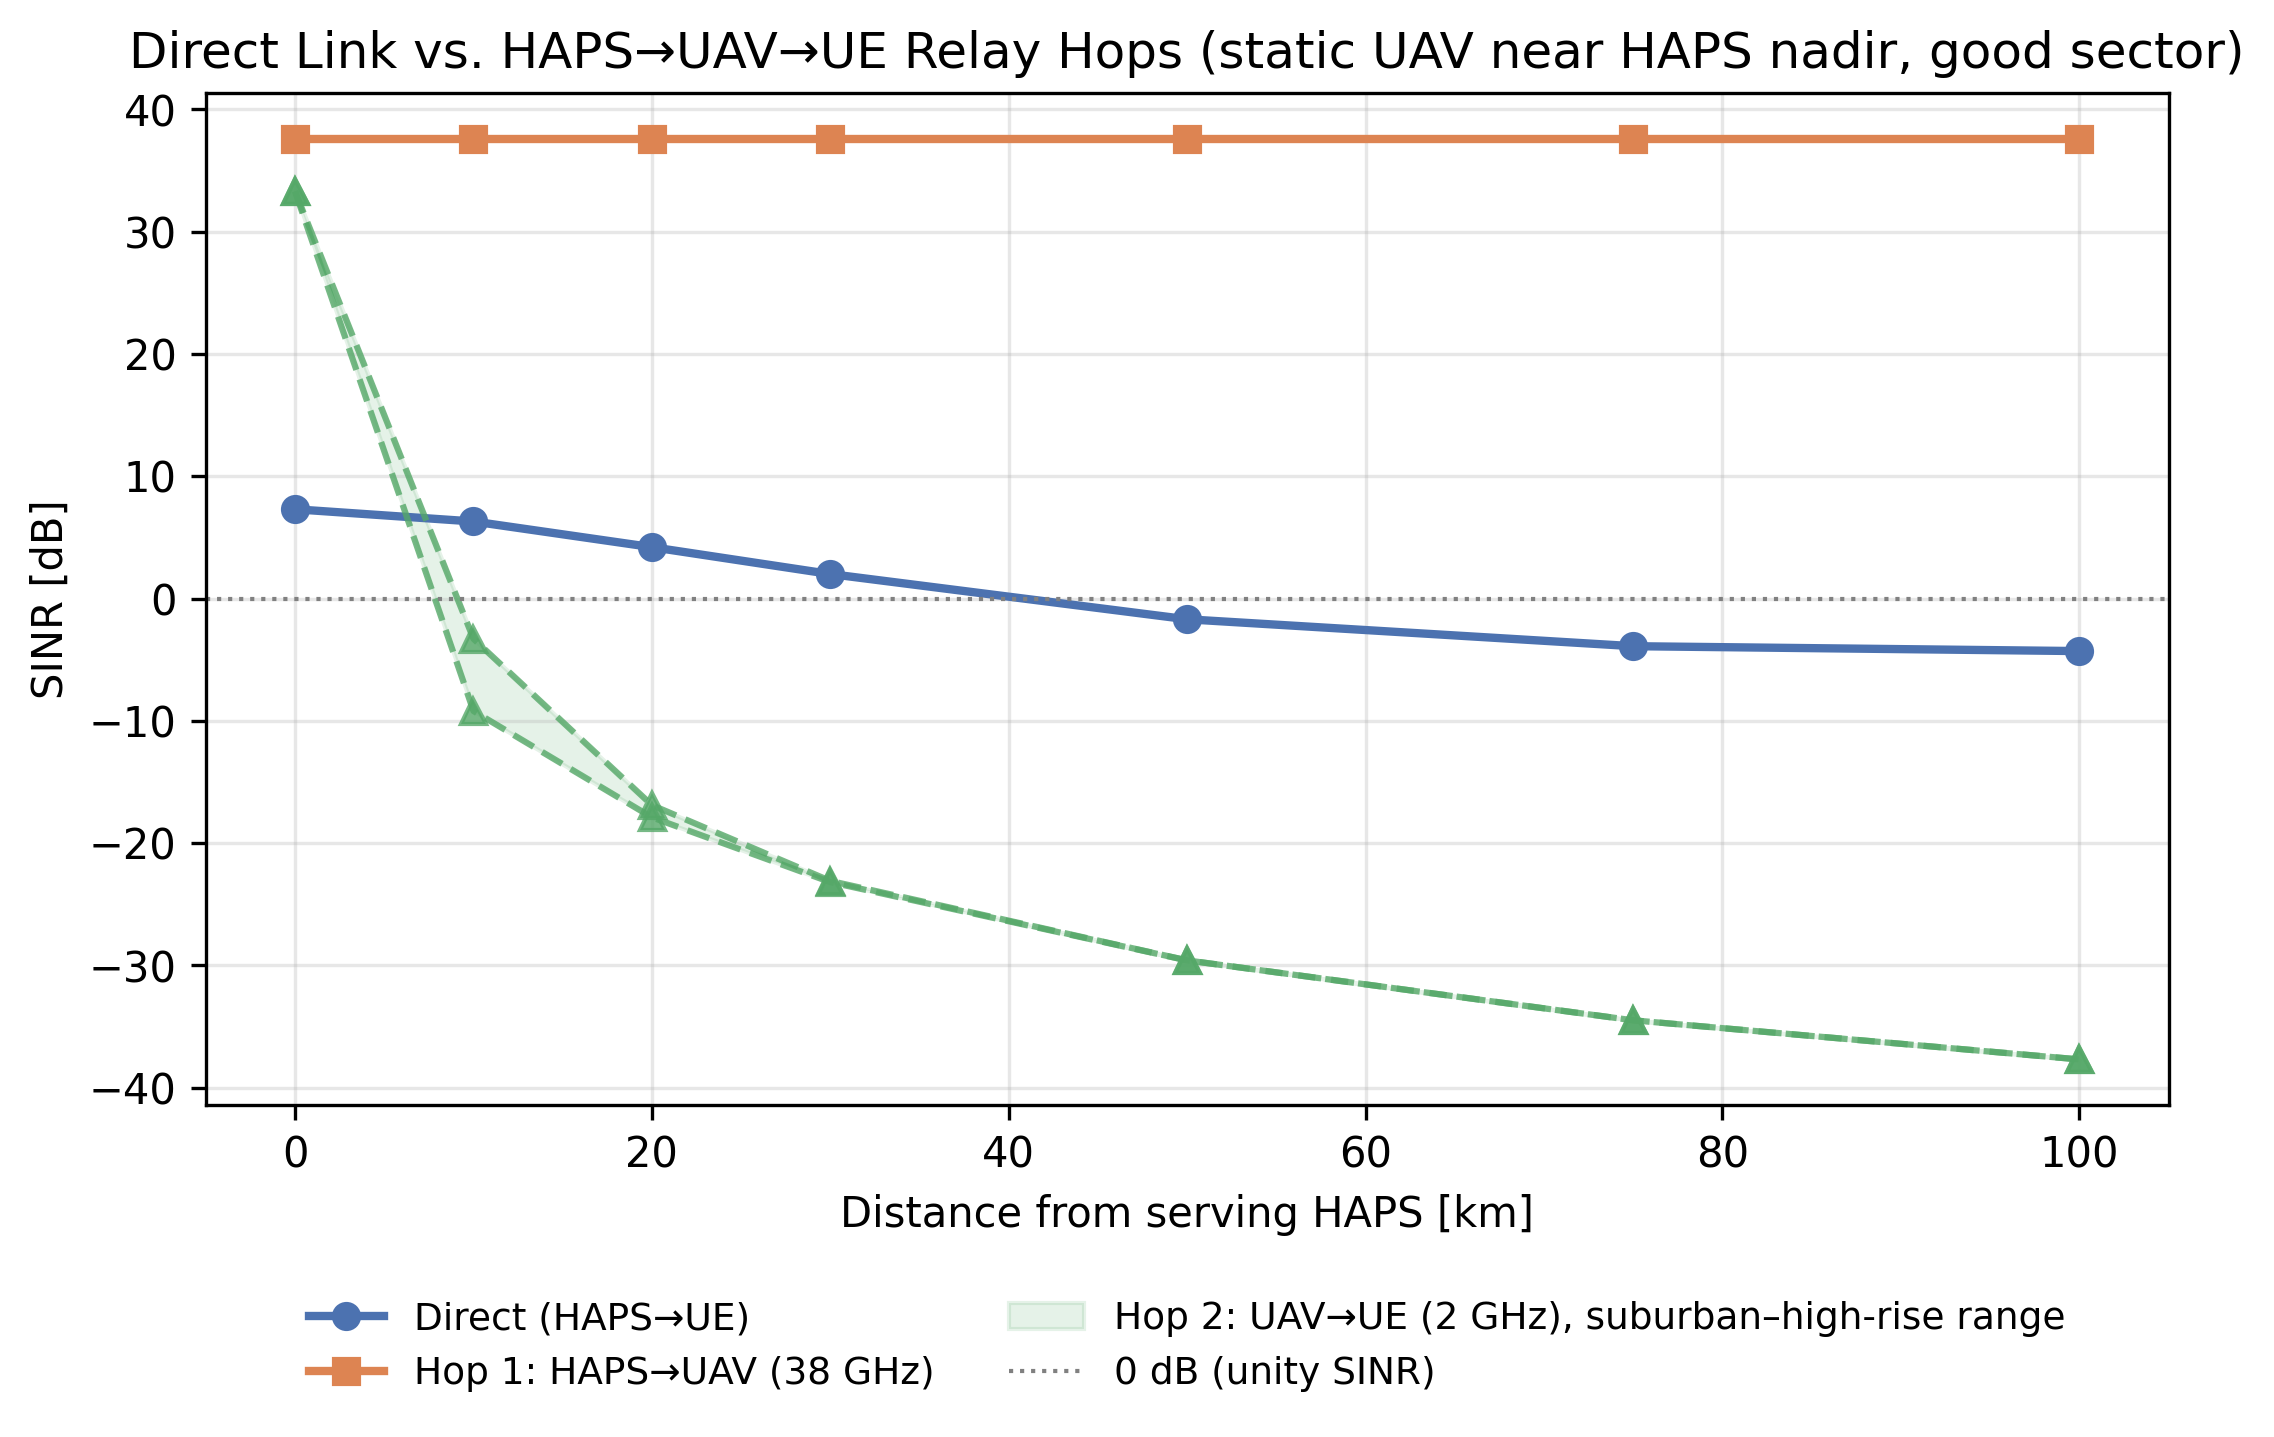
\includegraphics[width=0.95\columnwidth]{./figures/12_uav_relay_comparison.png}
\caption{SINR vs.\ the user's distance from the serving HAPS, azimuth-averaged, for the direct link and both relay hops, with the UAV fixed 0.1\,km from the serving HAPS's own nadir (good-sector azimuth). The feeder hop (HAPS$\to$UAV, 38~GHz) is flat at $\approx+37.6$\,dB, since the UAV's own position does not move; the access hop (UAV$\to$UE, 2~GHz) instead falls with each user's real distance from that one fixed point, from $\approx+33.3$\,dB near the UAV to $-37.7$\,dB at 100\,km (\S\ref{sec:relay-path-analysis}).}
\label{fig:uav-relay-comparison}
\end{figure}

\begin{figure}[!t]\centering
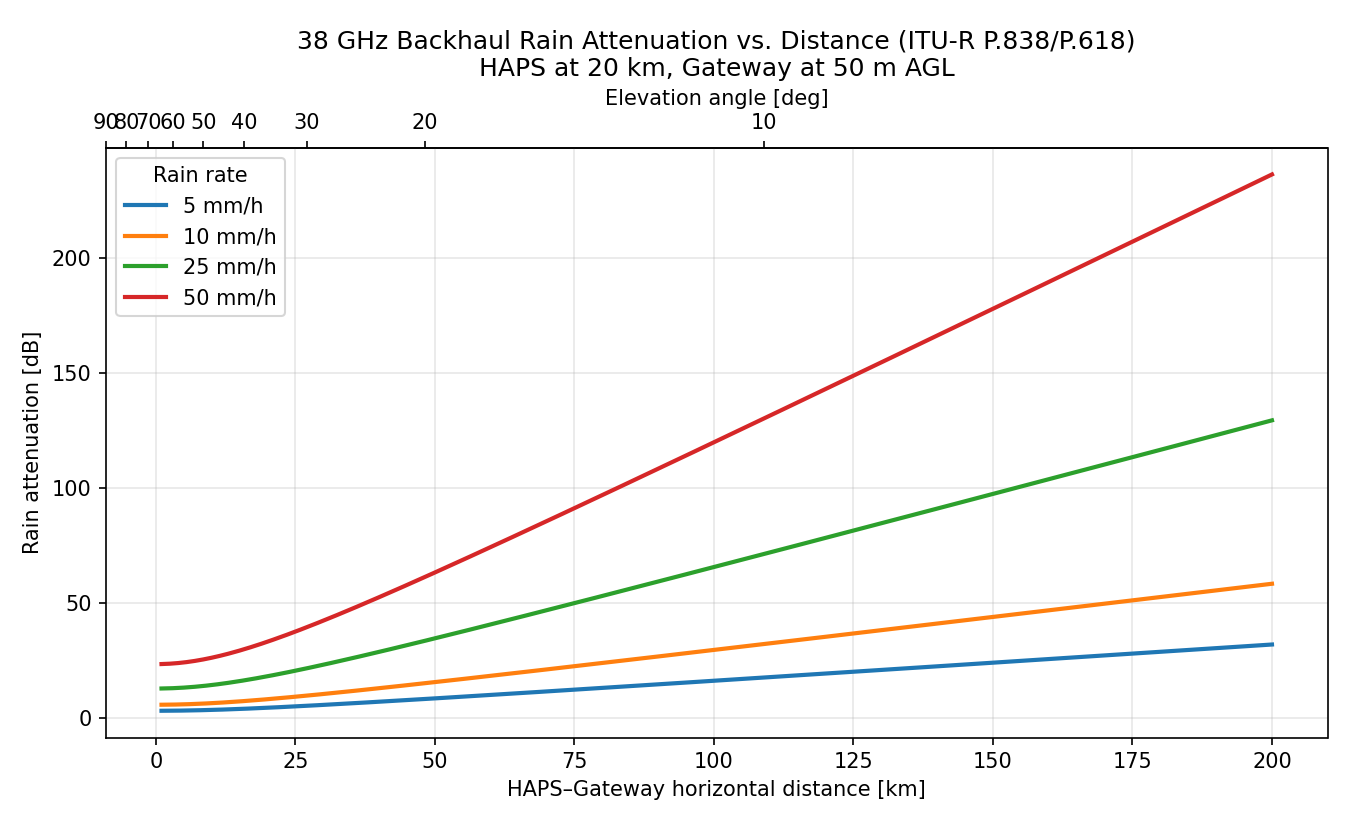
\includegraphics[width=0.95\columnwidth]{./figures/rain_attenuation_vs_distance.png}
\caption{38~GHz backhaul rain attenuation vs.\ HAPS--Gateway horizontal distance (ITU-R P.838/P.618), grows faster than linear past $\approx$100\,km as elevation drops and the slant path lengthens (\S\ref{subsec:backhaul-model}).}
\label{fig:rain-vs-distance}
\end{figure}

\subsection{Angular Interference Sectors and Scintillation}

\begin{figure}[!t]\centering
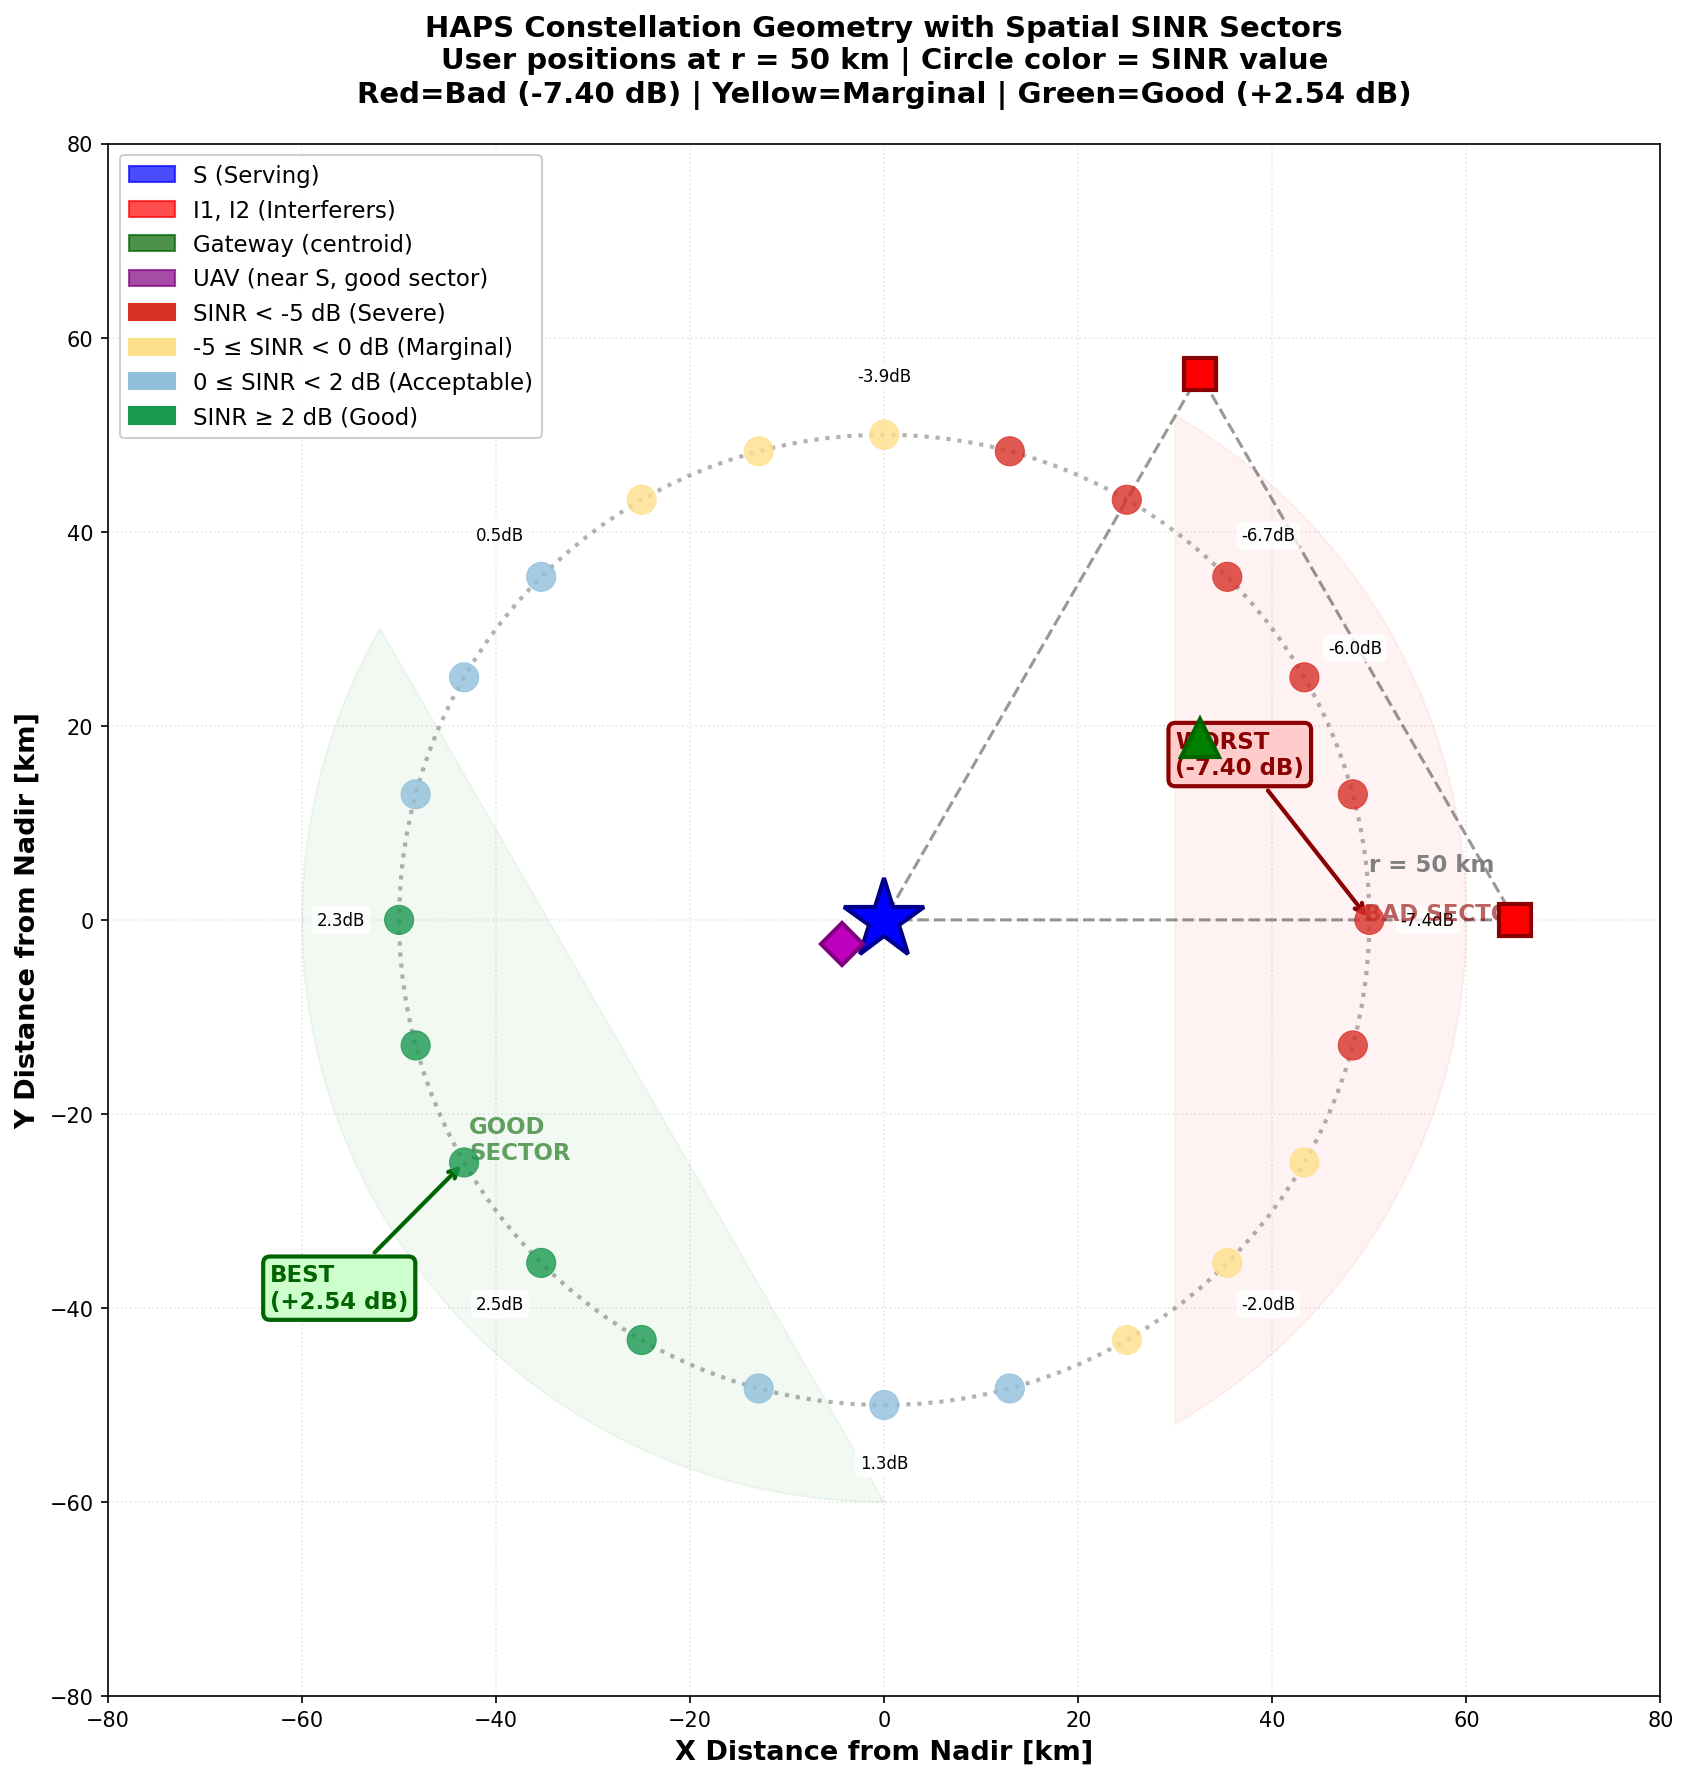
\includegraphics[width=0.85\columnwidth]{./figures/constellation_with_sectors.png}
\caption{HAPS constellation geometry (65\,km equilateral triangle: S at origin, I1 at $0^\circ$, I2 at $60^\circ$) with spatial SINR sectors at $r=50$\,km. Good sector (green, $\sim$120--290$^\circ$) vs.\ bad sector (red, $\sim$330--75$^\circ$). Best $+2.54$\,dB at $210^\circ$; worst $-7.40$\,dB at $0^\circ$.}
\label{fig:app-constellation-sectors}
\end{figure}

The good/bad-sector result of \S\ref{sec:multihaps} (Fig.~\ref{fig:app-constellation-sectors}) is one half of the angle- and weather-dependent picture; scintillation (Eq.~\eqref{eq:scint_loss}) is the other. At $30^\circ$ elevation, $p=0.01\,\%$, scintillation fade is $\approx$0.49\,dB at 38~GHz versus $\approx$0.09\,dB at 2.1~GHz -- growing with frequency and shrinking with elevation. Both effects favor positioning the UAV relay near nadir (higher elevation) when feasible, especially on the HAPS--UAV feeder hop, which also tends to fall in the interferer-facing sector's complement. This is not, however, a single clean optimization: each HAPS can simultaneously be a serving node (near-nadir, low-loss, for its own users) and an interferer for the other two HAPS' users -- jointly optimizing positioning across both roles is left to future work (\S\ref{sec:conclusion}).

\subsection{Why Learning Is Needed: Spatial SINR Heterogeneity}

\begin{figure}[!t]\centering
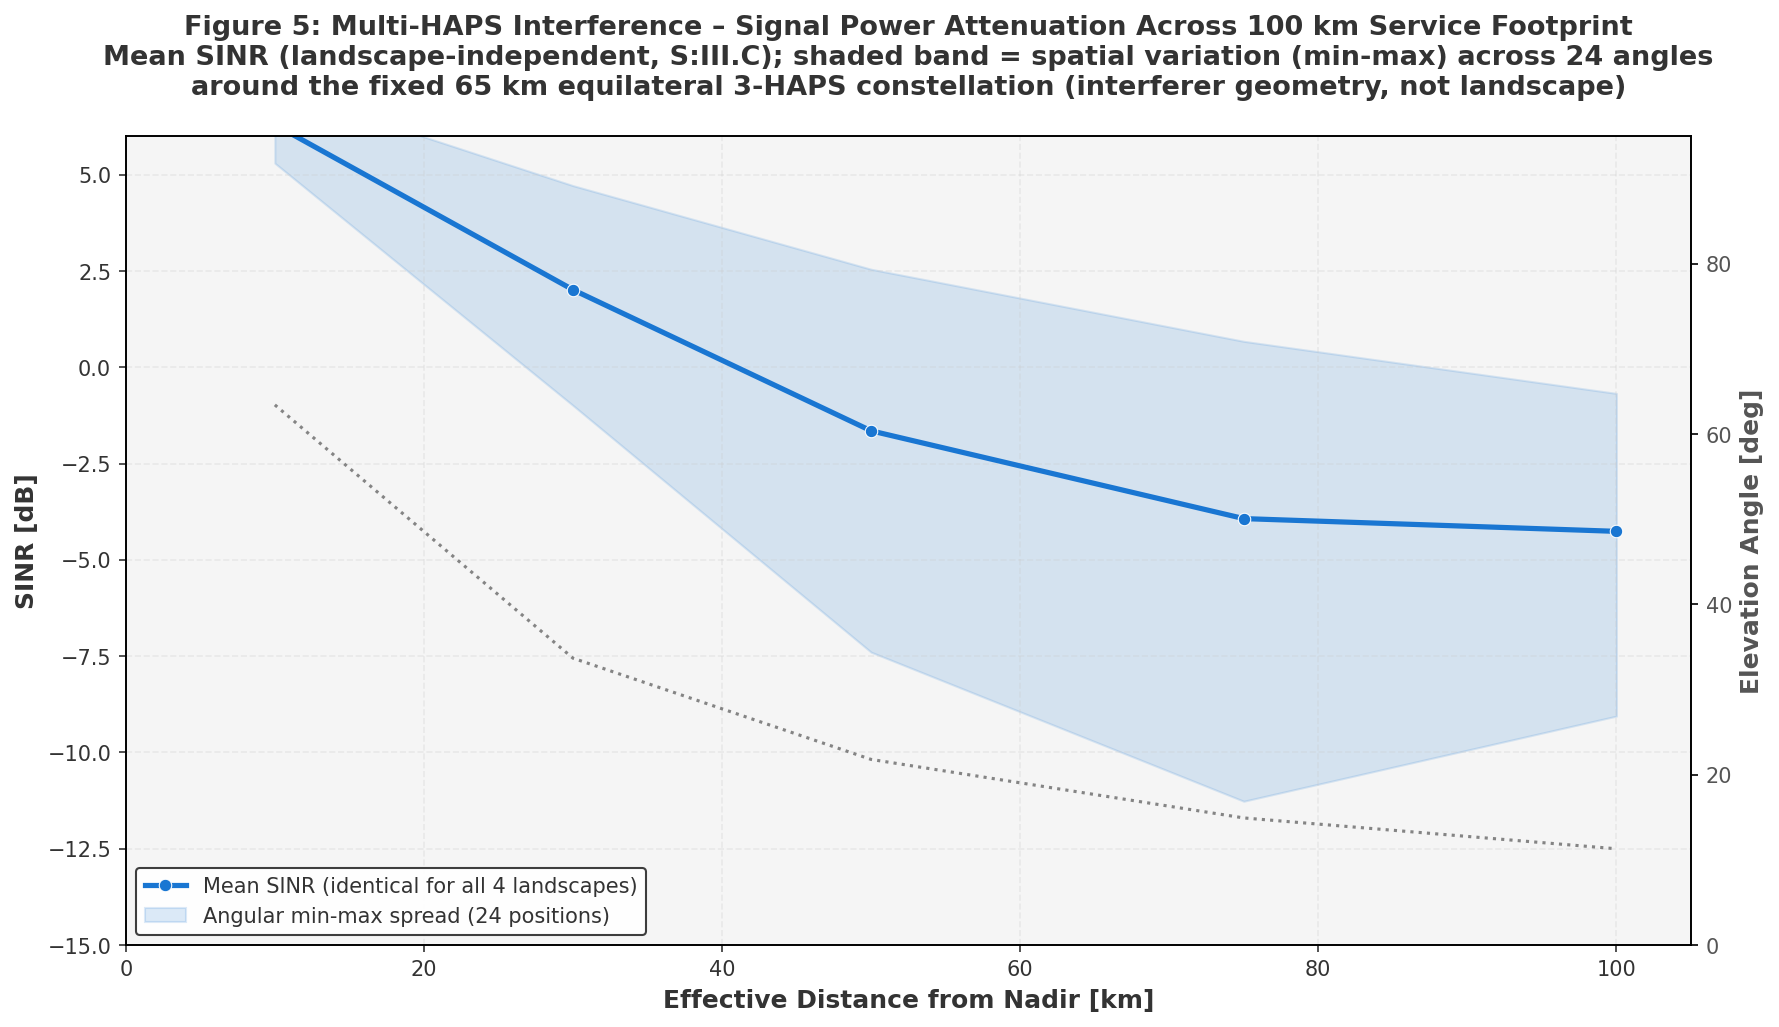
\includegraphics[width=0.95\columnwidth]{./figures/figure5_multi_haps_sinr_mean.png}
\caption{Mean SINR and angular min--max spread across the 100\,km service footprint: falls from $+6.3$\,dB at 10\,km to $-4.3$\,dB at 100\,km, while the spread widens to 11.94\,dB at 75\,km.}
\label{fig:multinode-interference}
\end{figure}

At a fixed 50~km radius, SINR varies by up to 9.94\,dB with angular position (\S\ref{sec:multihaps}), while doubling the link distance costs only $\sim$2--3\,dB -- angular position affects SINR more than distance does. A simple ``always pick max-SINR'' rule cannot anticipate these angular patterns or adapt as weather and battery state change, motivating a learned, real-time association policy.

\subsection{Stage 2: Baseline Association Policies}
\label{sec:baseline-policies}

Before introducing a learned policy, three rule-based (non-learned) association policies are evaluated on the channel model above, to establish how much association choice alone -- without any learning -- already changes outcomes. Each of $N$ users chooses one of six options every hour: a direct link to HAPS1--3, or a UAV relay via HAPS1--3 (\S\ref{sec:relay-path-analysis}).

\begin{itemize}\setlength{\itemsep}{1pt}
  \item \textbf{Random}: uniform-random choice among the six options each hour (sanity floor).
  \item \textbf{Max-SINR}: always the best-SINR \emph{direct} link (Eq.~\eqref{eq:sinr}); cannot use the relay, no memory of battery or fairness state.
  \item \textbf{Max-throughput}: the highest-throughput option among all six every hour, assuming perfect, instantaneous knowledge of every option's SINR and capacity -- a theoretical upper bound, not a deployable policy.
\end{itemize}

These three policies are carried forward as the baselines in \S\ref{sec:dqn-results}, where they are compared against the learned LSTM+DQN policy of \S\ref{sec:dqn} on the same held-out days and the same six-action set.

% =====================================================================
\section{LSTM Rain-Attenuation Forecaster}
\label{sec:lstm}
% =====================================================================

The DQN must choose an association at hour $t$ before that hour's rain is observed, so it needs a forecast of the feeder loss. An LSTM is trained to map the past 24 hours of weather (14 features: temperature, humidity, pressure, wind, precipitation, cloud amount, visibility, rain/fog codes, cloud liquid water, and sine/cosine encodings of time-of-day and season, from hourly NASA POWER, METAR and ERA5 data for Delhi, 2023--2026) to the next six hourly values of HAPS-to-gateway rain attenuation (38~GHz, $27.995^\circ$ elevation, Gateway fixed at the HAPS triangle's centroid, ITU-R P.838/P.618) -- the only link in this model where rain is a significant, time-varying impairment (\S\ref{subsec:service-model}); the 2~GHz service/relay link's rain, fog, and gas loss are negligible, so no forecast is needed there. Forecasts are always evaluated out-of-sample (e.g.\ 2026 forecasts from a model trained only on 2023--2025), and a forecast for hour $t$ is issued at $t-1$, so the agent never sees the rain of the hour it is acting on. In deployment this would be a continuous, incremental feed, with the model updating as new weather data arrives.

\begin{table}[t]
\centering
\caption{LSTM against persistence on 2026 (6557 forecast hours, no 2026 data in training): MAE/RMSE in dB per horizon. Bold marks the better method.}
\label{tab:lstm-2026}
{\scriptsize\setlength{\tabcolsep}{3pt}
\begin{tabularx}{\columnwidth}{|>{\centering\arraybackslash}X|>{\centering\arraybackslash}X|>{\centering\arraybackslash}X|>{\centering\arraybackslash}X|>{\centering\arraybackslash}X|}
\hline
\textbf{Horizon} & \textbf{LSTM MAE} & \textbf{Persist.\ MAE} & \textbf{LSTM RMSE} & \textbf{Persist.\ RMSE} \\
\hline
$+1$\,h & $0.20$ & $\mathbf{0.12}$ & $0.65$ & $\mathbf{0.53}$ \\
\hline
$+2$\,h & $0.27$ & $\mathbf{0.20}$ & $0.86$ & $\mathbf{0.75}$ \\
\hline
$+3$\,h & $0.31$ & $\mathbf{0.26}$ & $0.96$ & $\mathbf{0.90}$ \\
\hline
$+4$\,h & $0.33$ & $\mathbf{0.30}$ & $\mathbf{1.00}$ & $1.02$ \\
\hline
$+5$\,h & $0.34$ & $0.34$ & $\mathbf{1.00}$ & $1.11$ \\
\hline
$+6$\,h & $\mathbf{0.35}$ & $0.36$ & $\mathbf{1.02}$ & $1.17$ \\
\hline
\end{tabularx}}
\end{table}

Persistence is more accurate on RMSE at $+1$ to $+3$\,h and on MAE at $+1$ to $+4$\,h; the LSTM is more accurate on RMSE at $+4$ to $+6$\,h, and on MAE it ties persistence at $+5$\,h and wins at $+6$\,h (Table~\ref{tab:lstm-2026}). The DQN's state uses all six forecast horizons regardless, since the gain is not uniform across horizons but the longer horizons matter most for pre-emptive rerouting. \textbf{Observation:} simply averaging the LSTM and persistence forecasts beats both alone on RMSE at \emph{every} horizon tested, not only on average -- e.g.\ $0.511$ vs.\ $0.645$ LSTM-only and $0.530$ persistence-only at $+1$\,h, widening to $0.966$ vs.\ $1.017$ and $1.171$ at $+6$\,h -- a consistent, verified effect, not an artifact of one horizon or one averaging choice.

\textbf{Does the forecast help the DQN itself?} A forecast ablation, trained and evaluated with the same ten-seed, 2400-episode protocol as \S\ref{sec:dqn-results} (\texttt{lstm} vs.\ a \texttt{none} variant with the six forecast features zeroed, and an \texttt{oracle} variant given the true future attenuation) finds the forecast does not help, and at conventional significance ($\alpha=0.05$), slightly \emph{hurts}: \texttt{lstm} is worse than \texttt{none} ($-0.38$ reward/step, $p=0.022$, better in only $1/10$ seeds), while \texttt{lstm} vs.\ \texttt{oracle} and \texttt{none} vs.\ \texttt{oracle} are not significant ($p=0.17$, $p=0.70$). The forecast's own accuracy (above) and its value to the trained association policy are therefore separate questions, and only the first is a clear win here; forecast ensembling remains the better-supported, verified contribution of this section, noted further in \S\ref{sec:conclusion}.

\begin{figure}[t]
\centering
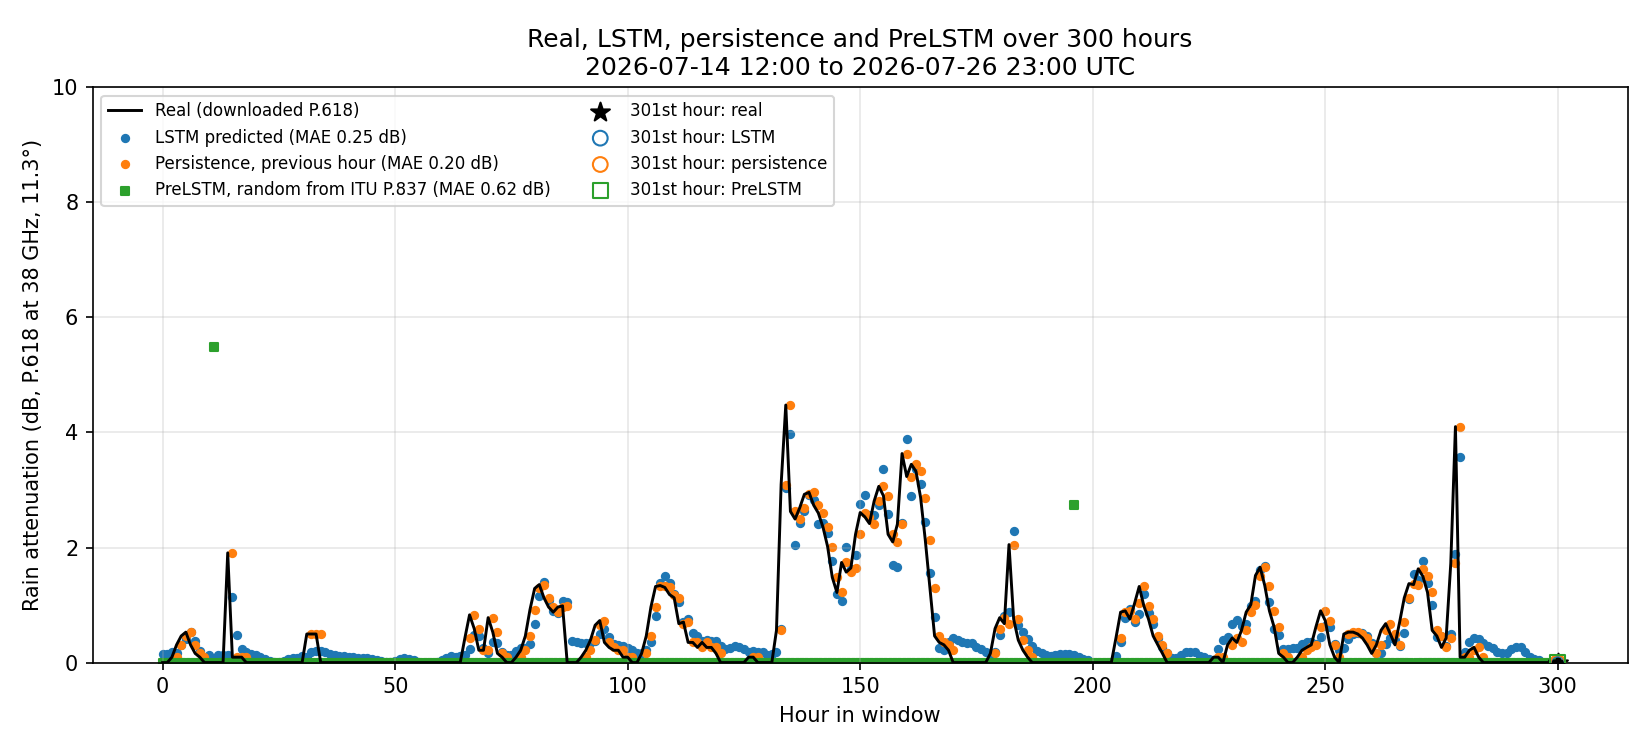
\includegraphics[width=\linewidth]{./figures/lstm_forecast_2026.png}
\caption{Real, LSTM, persistence and a synthetic PreLSTM baseline over a 300-hour window in July 2026 (the window with the most rain). LSTM: one-hour-ahead forecast. Persistence: previous hour's value. PreLSTM: random hourly rain rates drawn from ITU-R P.837 statistics, converted via P.618.}
\label{fig:lstm-2026}
\end{figure}

% =====================================================================
\section{DQN Association Agent}
\label{sec:dqn}
% =====================================================================

\subsection{Per-User MDP Formulation}

Each of the three platforms can serve a user directly or through the UAV relay, giving six actions $a_k\in\{0,\dots,5\}$ (actions 0--2: direct HAPS1--3; actions 3--5: UAV relay via HAPS1--3). With $N$ users, a centralized MDP over joint assignments is intractable, so the problem decomposes into per-user MDPs: each user independently chooses a platform, and reward is computed after all assignments.

With a single, static relay UAV (Table~\ref{tab:config}), choosing \emph{which} HAPS feeds the UAV's feeder hop is folded into this same per-user action set, effectively treating the UAV as if it were just another user requesting a serving HAPS. Only the \emph{shape} of that choice is shared (pick one of three HAPS) -- the channel model evaluating it is not: the UAV's feeder hop still uses the 38~GHz, ITU-R-P.618 feeder model of \S\ref{subsec:backhaul-model} (its own antenna gains and atmospheric terms), never the 2~GHz building-blockage model of \S\ref{subsec:service-model} that a direct user's choice is evaluated against. Sharing the action's shape, not its physics, is a fair simplification when there is only one UAV to assign. This does not generalise to a UAV fleet: at fleet scale, UAV-to-HAPS assignment (an $O(\text{fleet size})$ problem, e.g.\ the $\sim$200-UAV deployment of \S\ref{sec:conclusion}) and UE-to-UAV/HAPS access (an $O(N)$ problem) become two separably-sized assignment problems that cannot stay bundled into one per-user action, since the UAV side would then be a shared resource contended for by many users' decisions at once rather than belonging to any single user's action space.

\textbf{State} (per user, 21-dimensional): SINR to each platform (dB, Eq.~\eqref{eq:sinr}), horizontal distance to each (km), each HAPS's battery state of charge (\%, \S\ref{subsec:battery}), the UAV-relay capacity to each platform (bits/s/Hz, \S\ref{sec:relay-path-analysis}), rainfall rate, visibility, time-of-day, and the six LSTM rain forecasts $\hat{A}_t,\dots,\hat{A}_{t+5}$ (\S\ref{sec:lstm}), issued at $t-1$ so no rain of hour $t$ enters the state. Tropospheric scintillation (\S\ref{subsec:backhaul-model}) is not included as a state feature -- it is a smaller, time-varying effect ($\le$0.6\,dB at 38~GHz, $p=1\,\%$) whose forecasting is left to future work.

\textbf{Reward.} For user $k$ with linear SINR $\gamma_k=10^{\mathrm{SINR}_{k,\mathrm{dB}}/10}$ on its chosen link,
\begin{align}
r_k &= \omega_1 T_k c_\mathrm{rain} + P^\mathrm{sev}_k + P^\mathrm{deg}_k + \omega_2 J_\mathrm{fair} - \omega_3 P_\mathrm{eng} + P_\mathrm{LB},\nonumber\\
T_k &= \log_2(1+\gamma_k), \qquad c_\mathrm{rain}=10^{-A_\mathrm{rain}/10}\in[0.05,1],\nonumber\\
J_\mathrm{fair} &= \frac{(\sum_k\gamma_k)^2}{N\sum_k\gamma_k^2}, \qquad P_\mathrm{eng}=\frac{1}{3}\sum_{p=1}^3\Big(1-\frac{\mathrm{SoC}_p}{100}\Big),
\label{eq:reward}
\end{align}
with $\omega_1=0.5,\omega_2=0.3,\omega_3=0.2$; $c_\mathrm{rain}$ de-rates every user's throughput credit alike, whether served directly or via the UAV relay, because all traffic -- direct or relayed -- ultimately transits the rain-faded 38~GHz backhaul to reach the core network (\S\ref{sec:topology}). $c_\mathrm{rain}$ leaves the other reward terms (fairness, outage, energy) untouched. Penalties (per user): severe outage $P^\mathrm{sev}_k=-100$ if $\mathrm{SINR}_{k,\mathrm{dB}}<-2$\,dB; degraded service $P^\mathrm{deg}_k=-20$ if $-2\le\mathrm{SINR}_{k,\mathrm{dB}}<0$\,dB; and a shared low-battery penalty $P_\mathrm{LB}=-50$ for any platform with $\mathrm{SoC}_p<10\,\%$ and at least one assigned user. The reported fairness metric (Jain index~\cite{jain1984quantitative} over per-user delivered throughput, $T_kc_\mathrm{rain}$) differs from $J_\mathrm{fair}$ above, which is Jain over linear SINR and enters only the reward.

\subsection{Battery Model}
\label{subsec:battery}

Each HAPS's battery state of charge (SoC) is tracked hourly,
\begin{equation}
\Delta\mathrm{SoC} = \frac{P_\mathrm{solar}(t) - (P_\mathrm{backhaul}+P_\mathrm{payload}+\sum_k P_{k,\mathrm{user}})}{C_\mathrm{battery}},
\label{eq:battery-balance}
\end{equation}
with $P_\mathrm{backhaul}=500$\,W, $P_\mathrm{payload}=200$\,W, and $C_\mathrm{battery}=12\,000$\,Wh. Because the HAPS operates above $>$99\,\% of clouds, solar generation is independent of ground weather and follows a diurnal cosine profile,
\begin{equation}
I_0(t_\mathrm{hr}) = \begin{cases} 600\cos\!\big(\pi(t_\mathrm{hr}-12)/12\big) & 6\le t_\mathrm{hr}\le 18\\ 0 & \text{night}\end{cases}\ [\mathrm{W/m^2}],
\end{equation}
giving $P_\mathrm{solar}(t)=20\,\mathrm{m}^2\times0.20\times I_0(t)$, i.e.\ $2400$\,W at noon and $0$\,W at night. SoC is clipped to $[0,100]\,\%$; below $5\,\%$ the platform shuts down (no service), and below $10\,\%$ with assigned users the reward's low-battery penalty applies, so the agent must learn to balance load across platforms to avoid over-draining any one HAPS overnight.

% =====================================================================
\section{DQN Results}
\label{sec:dqn-results}
% =====================================================================

The three stage-2 baseline policies (\S\ref{sec:baseline-policies}: random, max-SINR, max-throughput) are now compared against the stage-3 LSTM+DQN agent (\S\ref{sec:dqn}) on the same held-out days and six-action set. The DQN is a custom PyTorch (\texttt{torch}/\texttt{torch.nn}) network, trained on 2400 rolling 24-hour episodes (cycling the 400 real 2024 episodes six times; 400 was the original budget, but with the UAV relay fix above making three of the six actions traps for most users, training needed longer to converge -- 400 episodes left reward still improving noisily) and evaluated on 50 held-out 2025 days, across ten experiments (random seeds).

\begin{table}[t]
\centering
\caption{Policy comparison, 50 held-out 2025 days, mean over ten experiments (std.\ dev.\ across experiments in parentheses). Jain is over per-user delivered throughput.}
\label{tab:dqn-all-policies}
{\scriptsize\setlength{\tabcolsep}{3pt}
\begin{tabularx}{\columnwidth}{|>{\raggedright\arraybackslash}X|>{\centering\arraybackslash}X|>{\centering\arraybackslash}X|>{\centering\arraybackslash}X|}
\hline
\textbf{Policy} & \textbf{Reward/step} & \textbf{Jain} & \textbf{Outage/50} \\
\hline
Random (six actions) & $-91.9\,(1.5)$ & $0.262\,(0.005)$ & $41.5\,(0.3)$ \\
\hline
Max-SINR (direct only) & $-13.8\,(1.7)$ & $\mathbf{0.865}\,(0.002)$ & $0.8\,(0.2)$ \\
\hline
Max-throughput (six actions) & $\mathbf{-13.5}\,(1.6)$ & $0.862\,(0.002)$ & $\mathbf{0.7}\,(0.2)$ \\
\hline
LSTM + DQN & $-14.4\,(1.8)$ & $0.859\,(0.005)$ & $1.3\,(0.3)$ \\
\hline
\end{tabularx}}
\end{table}

With the UAV relay correctly modeled as a single static platform (\S\ref{sec:relay-path-analysis}), the picture changes from an earlier version of this model that let the UAV hover beside whichever user it served: the random policy now suffers badly, since three of its six equally-likely actions are usually traps, and \textbf{LSTM+DQN no longer has the highest reward} (Table~\ref{tab:dqn-all-policies}) -- it is statistically indistinguishable from, and on raw reward slightly behind, both max-SINR and max-throughput (paired across the same ten seeds: $-0.60$ vs.\ max-SINR, $p<0.0001$, $0/10$ seeds favoring the DQN; $-0.94$ vs.\ max-throughput, $p<0.0001$, $0/10$). Decomposing the reward by term (throughput, fairness, and battery energy are statistically tied across all three policies) shows the gap is driven almost entirely by a higher severe-outage rate: the DQN leaves users in severe outage ($\mathrm{SINR}<-2$\,dB) on $2.5\,\%$ of user-hours, against $1.3$--$1.7\,\%$ for the two rule-based policies, which by construction never choose worse than the best currently-visible direct option. Max-SINR needs only a real-time SINR measurement, already a deployable rule; max-throughput, which additionally compares all six options' instantaneous capacity including relay, needs perfect, instantaneous knowledge of capacities it cannot actually measure non-causally, but since relay rarely wins post-fix, it also collapses in practice to "pick the best direct option." Despite this, the DQN is the only policy that retains and actually uses the relay path: it invokes relay specifically for users whose best direct SINR already averages $-1.9$\,dB (population mean $+2.4$\,dB), consistent across all ten seeds ($p=1.3\times10^{-13}$) -- a targeted, structural use of relay capacity that neither rule-based baseline can replicate, since Max-SINR cannot use relay at all and Max-throughput's instantaneous rule has no notion of \emph{which} users most need it.

\begin{figure}[t]
\centering
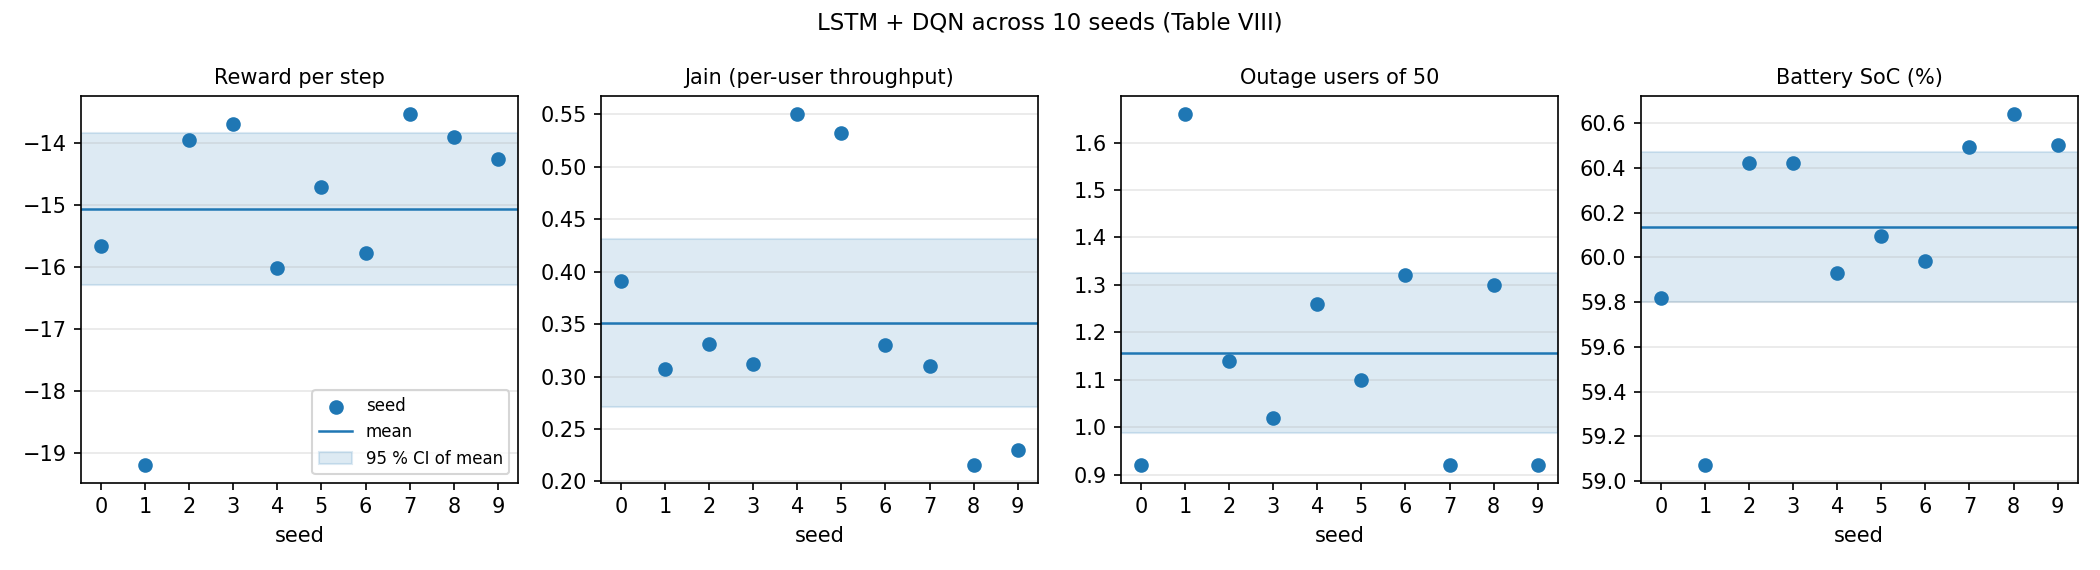
\includegraphics[width=\linewidth]{./figures/seed_stats.png}
\caption{LSTM+DQN, ten independent seeds (dot = one training run; line = mean; band = 95\,\% CI of the mean). Reward/step $-14.44\pm1.76$ (95\,\% CI $[-15.69,-13.18]$); Jain $0.859\pm0.005$; outage $1.30\pm0.28$ of 50 users; battery SoC $60.14\pm0.47\,\%$. The shaded band narrows with more seeds and reflects precision of the estimated mean, not run-to-run spread; the tight spread across all ten seeds shows the policy is reliably learned to this level, not a lucky or unlucky single run -- consistency, not the reward level itself, is what this figure demonstrates.}
\label{fig:seed-stats}
\end{figure}

\begin{figure}[t]
\centering
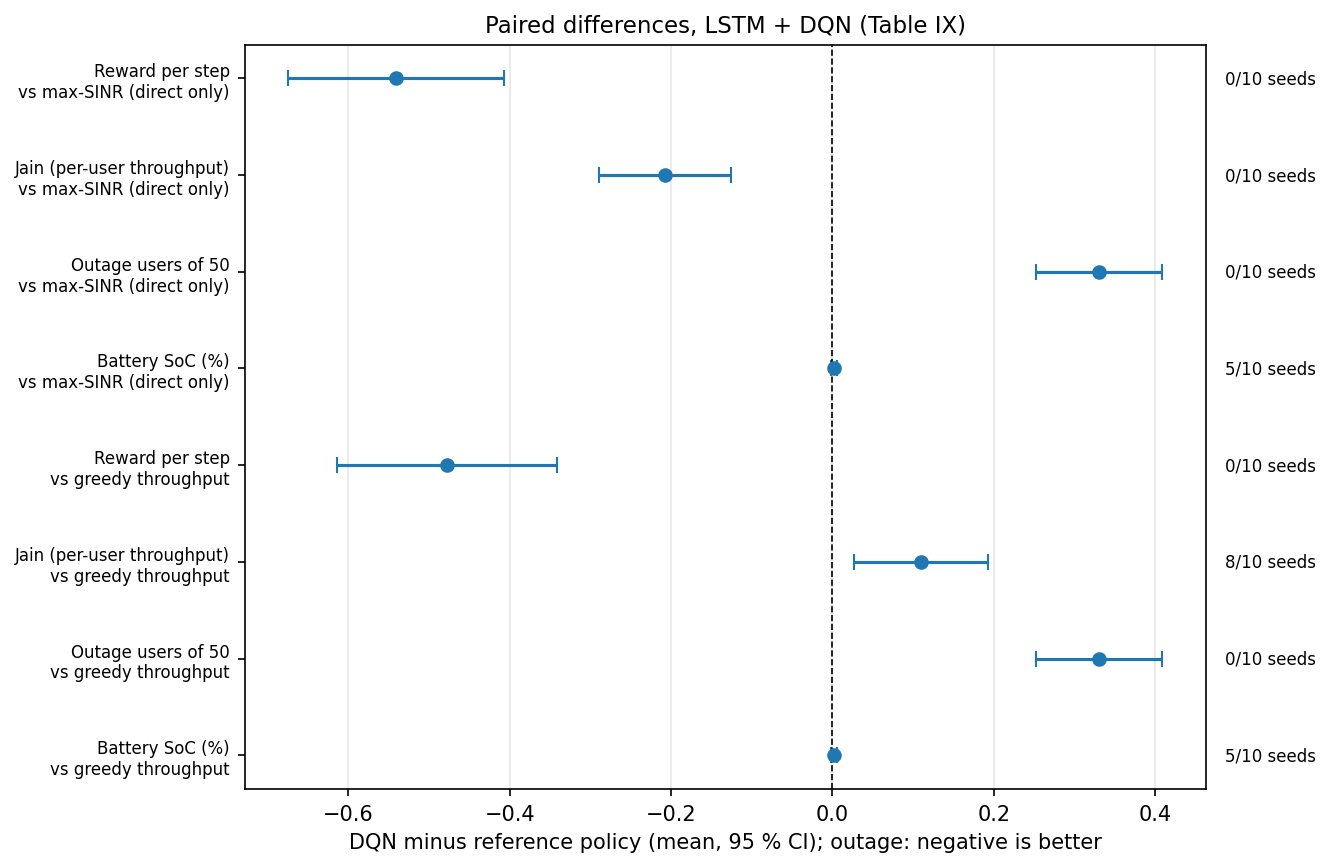
\includegraphics[width=\linewidth]{./figures/paired_forest.png}
\caption{Paired differences, LSTM+DQN minus baseline, per experiment (50 days each, ten seeds); whiskers crossing zero are not significant. Vs.\ max-SINR: reward $-0.60$ ($p<0.0001$, $0/10$ seeds favoring DQN), Jain $-0.0065$ ($p=0.0008$, $0/10$), outage $+0.48$, i.e.\ worse ($p=0.0002$, $0/10$), battery SoC $\approx0$ ($p=0.68$, tie). Vs.\ max-throughput: reward $-0.94$ ($p<0.0001$, $0/10$), Jain $-0.0029$ ($p=0.08$, tie), outage $+0.65$, i.e.\ worse ($p<0.0001$, $0/10$), battery SoC $\approx0$ ($p=0.35$, tie). The DQN now loses to both rule-based policies on reward and outage on every seed, and ties (never beats) them on fairness and battery; \S\ref{sec:dqn-results} decomposes this gap and the relay-targeting behaviour that nonetheless distinguishes the DQN from either baseline.}
\label{fig:paired-forest}
\end{figure}

% =====================================================================
\section{Conclusion}
\label{sec:conclusion}
% =====================================================================

This paper characterised the HAPS--UAV--Gateway air-to-ground channel across its three link types, quantified multi-HAPS interference and the UAV-relay path as an alternative to the direct service link, and used that channel model to train and evaluate a DQN association agent.

\textbf{Channel model.} Spatial SINR heterogeneity -- up to 9.94\,dB at a fixed 50\,km radius, driven by angular position relative to the two interfering HAPS -- dominates service-link quality; the backhaul link remains noise-limited and largely unaffected by constellation geometry.

\textbf{Relay path.} With the single relay UAV correctly modeled as static (\S\ref{sec:relay-path-analysis}), now fixed 0.1\,km from the serving HAPS's own nadir (the Gateway occupies the centroid instead), its feeder hop is reliably flat ($12.48$\,bits/s/Hz, $\approx$89.71$^\circ$ elevation, the same for every HAPS by the constellation's symmetry) but its access hop collapses within a few kilometres of that one fixed point, far faster than the direct link degrades with distance from a HAPS. Averaged over azimuth, relay capacity now exceeds the direct link's within about 1--2\,km (urban) to 5--6\,km (suburban) of the serving HAPS's own nadir -- where the fixed UAV happens to sit -- but falls back below it for the rest of its $\approx$6.5--10.3\,km usable radius, so area-averaged over that whole radius the relay delivers \emph{less} capacity than the direct link does over the same disk ($\approx0.79$--$0.87\times$), the opposite of the previous centroid-UAV finding. A single static UAV therefore helps only a small minority of users, and -- now that its own disk largely overlaps the direct link's own best-served area near the HAPS nadir -- a useful fleet would need to be placed \emph{away} from each HAPS's own nadir instead; a covering-number estimate for disks of this same $\approx$6.5\,km radius still puts full, gap-free coverage of the 100\,km service radius at $\sim$200--270 such UAVs (\S\ref{sec:dqn} discusses why that is a separate fleet-assignment problem, not a scaled-up version of today's single-UAV model). The direct service link itself does not scale to replace this: it has no modeled mechanism for sharing its narrow band across many simultaneous users, unlike the feeder link, which is inherently wideband and aggregates traffic the way terrestrial backhaul does. Both links are, in that sense, best read as a wide-area, low-infrastructure fallback (direct) and a capacity-scalable but currently under-deployed primary path (relay), rather than the direct link being primary and relay the backup, as a single static UAV's limited reach might otherwise suggest.

\textbf{Learned association.} With the relay path corrected, the LSTM-fed DQN is statistically indistinguishable from, and on raw reward and outage slightly behind, both max-SINR and max-throughput -- a reversal of an earlier result obtained under the unrealistic always-nearby-UAV assumption. The gap traces to a higher severe-outage rate, not to throughput, fairness or battery management, on which all three tie. The forecast itself shows no measurable reward benefit, and is slightly, significantly worse than no forecast at all under a matched training budget (\S\ref{sec:dqn-results}), though it remains the more accurate forecaster on its own terms (\S\ref{sec:lstm}). What distinguishes the DQN is structural, not a reward-table win: it is the only policy that retains and actually uses the relay path, and it does so as a targeted fallback for users already near the outage threshold, not indiscriminately -- a capability neither rule-based baseline can have, since Max-SINR cannot use relay at all and Max-throughput's instantaneous rule has no notion of which specific users need it most.

\textbf{Roadmap for future investigations.} (i) This paper already shows relaying is worthwhile mainly within $\approx$6.5\,km of the single UAV, and the DQN learns to target it there (\S\ref{sec:dqn-results}); open is learning this jointly with \emph{which} HAPS feeds the UAV once that becomes a real choice (multiple, non-equidistant UAVs); (ii) model movement of the HAPS and UAV platforms; (iii) consider more UAVs, including UAV selection -- at fleet scale this should split into two separate MDPs (\S\ref{sec:dqn}: UAV-to-HAPS assignment and UE-to-access-point assignment), with relay-vs-direct decided as its own explicit policy rather than folded into a single per-user choice, and with UAV placement itself chosen to avoid the blind-corner coverage gaps a naive non-overlapping tiling leaves behind, reducing the resulting edge-of-coverage errors; (iv) extend the LSTM forecast to neighbouring regions (e.g.\ a ConvLSTM on gridded reanalysis data, or a spatio-temporal graph model such as DCRNN, T-GCN or Graph WaveNet, if future sites are irregularly placed); (v) adapt to changing HAPS roles, shifting a node between serving and interfering based on its distance to the gateway, and jointly optimize UAV/HAPS positioning across both roles a node could play at once, rather than each in isolation; (vi) consider beamforming between HAPS and gateway; and (vii) explore forecast ensembling further -- averaging the LSTM and persistence forecasts already improves RMSE at every horizon tested (\S\ref{sec:lstm}), even though the forecast alone does not yet measurably improve the association policy's reward.

\section{Abbreviations}
\begin{tabular}{ll}
\textbf{ABS} & Aerial Base Station \\
\textbf{AGL} & Above Ground Level \\
\textbf{CDF} & Cumulative Distribution Function \\
\textbf{DRL} & Deep Reinforcement Learning \\
\textbf{DQN} & Deep Q-Network \\
\textbf{FDMA} & Frequency Division Multiple Access \\
\textbf{FSPL} & Free-Space Path Loss \\
\textbf{GW} & Gateway \\
\textbf{HAPS} & High-Altitude Platform Station \\
\textbf{ITU} & International Telecommunication Union \\
\textbf{K-band} & 18--27 GHz (ITU-R P.618 scintillation model) \\
\textbf{Ka-band} & 27--40 GHz (Scaled from K-band via $(f/20)^{0.7}$) \\
\textbf{LoS} & Line-of-Sight \\
\textbf{LSTM} & Long Short-Term Memory \\
\textbf{LWC} & Liquid Water Content \\
\textbf{MDP} & Markov Decision Process \\
\textbf{MLP} & Multi-Layer Perceptron \\
\textbf{MVP} & Minimum Viable Product \\
\textbf{NLoS} & Non-Line-of-Sight \\
\textbf{PDF} & Probability Density Function \\
\textbf{PL} & Path Loss \\
\textbf{RH} & Relative Humidity \\
\textbf{SINR} & Signal-to-Interference-plus-Noise Ratio \\
\textbf{SoC} & State of Charge (Battery) \\
\textbf{TDMA} & Time Division Multiple Access \\
\textbf{TD} & Temporal Difference \\
\textbf{UAV} & Unmanned Aerial Vehicle \\
\textbf{UTD} & Uniform Theory of Diffraction \\
\end{tabular}

\section{References}
% =====================================================================
% Sorted by publication year, latest first.
%\renewcommand{\refname}{}
\begin{thebibliography}{20}

\bibitem{liu2026multihaps}
\textbf{[2026]} S.~Liu, H.~Dahrouj, A.~Kammoun, and M.-S.~Alouini, ``Sum Rate and Worst-Case
SINR Optimization in Multi-HAPS--Ground Integrated Networks,'' \emph{IEEE
Trans. Aerosp. Electron. Syst.}, vol.~62, pp.~4540--4555, 2026.

\bibitem{svistunov2025haps}
\textbf{[2025]} G.~Svistunov, A.~Akhtarshenas, D.~L\'opez-P\'erez, M.~Giordani, G.~Geraci, and
H.~Yanikomeroglu, ``Bridging Earth and Space: A Survey on HAPS for
Non-Terrestrial Networks,'' \emph{IEEE Commun. Surveys Tuts.}, under review,
2025. arXiv:2510.19731.

\bibitem{karaman2025haps}
\textbf{[2025]} M.~Karaman et~al., ``On-Demand HAPS-Assisted Communication System for Public
Safety,'' \emph{IEEE Commun. Mag.}, 2025. arXiv:2507.09153.
[Table I: 38/30~GHz-class HAPS backhaul link budget -- Tx power 43.2~dBm,
Tx antenna gain 13.8~dBi, Gateway Rx antenna gain 39.7~dBi]

\bibitem{bakambekova2024}
\textbf{[2024]} A.~Bakambekova, N.~Kouzayha, and T.~Al-Naffouri, ``On the Interplay of Artificial
Intelligence and Space-Air-Ground Integrated Networks: A Survey,'' \emph{IEEE Open
J. Commun. Soc.}, vol.~5, pp.~4613--4673, 2024.

\bibitem{arani2023}
\textbf{[2023]} A.~H. Arani, P.~Hu, and Y.~Zhu, ``HAPS-UAV-Enabled Heterogeneous Networks: A Deep
Reinforcement Learning Approach,'' \emph{IEEE Open J. Commun. Soc.}, vol.~4,
pp.~1745--1760, 2023.
DOI: 10.1109/OJCOMS.2023.3294598

\bibitem{naous2023rlsky}
\textbf{[2023]} T.~Naous, M.~Itani, M.~Awad, and S.~Sharafeddine, ``Reinforcement Learning in
the Sky: A Survey on Enabling Intelligence in NTN-Based Communications,''
\emph{IEEE Access}, vol.~11, pp.~19941--19968, 2023.
DOI: 10.1109/ACCESS.2023.3249890

\bibitem{cornejo2022lstmrain}
\textbf{[2022]} A.~Cornejo, S.~Landeros, J.~M.~Mat\'ias, F.~G.~Ortiz-Gomez, R.~Mart\'inez, and
M.~A.~Salas-Natera, ``Method of Rain Attenuation Prediction Based on
Long--Short Term Memory Network,'' \emph{Neural Process. Lett.}, vol.~54,
no.~4, pp.~2959--2995, 2022.
DOI: 10.1007/s11063-022-10749-1

\bibitem{itu_p530}
\textbf{[2021]} ITU-R Recommendation P.530-17, ``Propagation data and prediction methods required
for the design of terrestrial line-of-sight systems,'' 2021.
Available: \url{https://www.itu.int/rec/R-REC-P.530/latest/}

\bibitem{itu_p618}
\textbf{[2021]} ITU-R Recommendation P.618-13, ``Propagation data and prediction methods for the
design of Earth-space telecommunication systems,'' 2021.
Available: \url{https://www.itu.int/dms_pubrec/itu-r/rec/p/R-REC-P.618-13-202108-S!!PDF-E.pdf}
[Covers rain attenuation reduction factors, slant-path geometry, scintillation model]

\bibitem{itu_p676}
\textbf{[2021]} ITU-R Recommendation P.676-12, ``Attenuation by atmospheric gases and related
effects,'' 2021.
Available: \url{https://www.itu.int/dms_pubrec/itu-r/rec/p/R-REC-P.676-12-202112-S!!PDF-E.pdf}
[Section 3.1.2: O$_2$ resonance (59.8 GHz, 118.75 GHz); Section 3.2.1: H$_2$O resonance (22.235 GHz)]

\bibitem{itu_p840}
\textbf{[2021]} ITU-R Recommendation P.840-6, ``Attenuation due to clouds and fog,'' 2021.
Available: \url{https://www.itu.int/dms_pubrec/itu-r/rec/p/R-REC-P.840-6-202101-I!!PDF-E.pdf}
[Liquid water content model for fog/cloud attenuation]

\bibitem{itu_p1410}
\textbf{[2021]} ITU-R Recommendation P.1410-5, ``Propagation data and prediction methods for the
design of terrestrial broadband radioaccess systems operating in a frequency range
from 3 to 60 GHz,'' 2021.
Available: \url{https://www.itu.int/rec/R-REC-P.1410/latest/}
[Elevation-angle-dependent LoS probability baseline]

\bibitem{anim2021uav}
\textbf{[2021]} E.~Anim, J.~Lee, and H.~Jung, ``High-Gain Millimeter-Wave Patch Array Antenna
for Unmanned Aerial Vehicle Application,'' \emph{Sensors}, vol.~21, no.~11,
p.~3914, 2021.
DOI: 10.3390/s21113914
[32x32 mmWave patch array: 30.7--32.8~dBi at 25.4--26.9~GHz]

\bibitem{sutton2018rl}
\textbf{[2018]} R.~S.~Sutton and A.~G.~Barto, \emph{Reinforcement Learning: An Introduction},
2nd~ed. Cambridge, MA: MIT Press, 2018.
[MDP theory, value functions, policy gradient methods; Chapter 6: Q-learning]

\bibitem{schulman2017ppo}
\textbf{[2017]} J.~Schulman, F.~Wolski, P.~Dhariwal, A.~Radford, and O.~Klimov,
``Proximal policy optimization algorithms,'' arXiv preprint arXiv:1707.06347, 2017.
[Policy-gradient alternative to DQN; higher sample complexity for discrete actions]

\bibitem{mnih2015dqn}
\textbf{[2015]} V.~Mnih, K.~Kavukcuoglu D.~Silver, A.~A.~Rusu, J.~Veness, G.~Bellemare,
A.~Graves, M.~Riedmüller, A.~K.~Fidjeland, G.~Ostrovski, S.~Petersen,
C.~Beattie, A.~Sadik, I.~Antonoglou, H.~King, D.~Kumaran, D.~Wierstra,
S.~Legg, and D.~Hassabis, ``Human-level control through deep reinforcement
learning,'' \emph{Nature}, vol.~529, pp.~529--533, 2015.
[Foundational DQN algorithm: experience replay, target networks, Q-learning]

\bibitem{ecc_report_156}
\textbf{[2011]} European Communications Committee (ECC), ``Minimum performance characteristics
for spectrum sharing between Fixed Satellite Service (FSS) and other services,''
ECC Report 156, April 2011 (updated December 2014).
Available: \url{https://www.ecc.cept.org/ecc/documents/ecc-reports/}
[Spectrum-sharing guidance; rain attenuation margins at Ka-band]

\bibitem{holispechac2008}
\textbf{[2008]} J.~Holis and P.~Pechac, ``Elevation Dependent Shadowing Model for Mobile
Communications via High Altitude Platforms in Built-up Areas,'' \emph{IEEE
Trans. Antennas Propag.}, vol.~56, no.~4, pp.~1078--1084, Apr. 2008.
DOI: 10.1109/TAP.2008.919209
[Building-blockage LoS probability series; environment parameters (Table I): $(\alpha, \beta, \xi)$ for suburban/urban/dense-urban/high-rise]

\bibitem{itu_p838}
\textbf{[2005]} ITU-R Recommendation P.838-3, ``Specific attenuation model for rain for use in
prediction methods,'' 2005.
Available: \url{https://www.itu.int/dms_pubrec/itu-r/rec/p/R-REC-P.838-3-200503-S!!PDF-E.pdf}
[Annex 1: frequency-dependent rain coefficients $k(f)$, $\alpha(f)$]

\bibitem{goldsmith2005}
\textbf{[2005]} A.~Goldsmith, \emph{Wireless Communications}, Cambridge University Press, 2005.
[Multi-user SINR in linear domain; noise and interference are additive in linear scale, not dB]

\bibitem{jain1984quantitative}
\textbf{[1984]} R.~K.~Jain et~al., ``A quantitative measure of fairness and discrimination for resource allocation in shared computer systems,''
\textit{arXiv preprint arXiv:cs/9809099}, 1984.

\end{thebibliography}


\EOD
\end{document}
